%------------------------------------------------------------------------------
% CHAPTER 3: SPECIFIC REQUIREMENTS
%------------------------------------------------------------------------------
\chapter{Specific Requirements}
\label{ch:requirements}

\section{External Interface Requirements}
\label{sec:interfaces}

\subsection{User Interfaces}

\begin{itemize}
    \item \textbf{Sign Up/Login Page}: The system must include a Sign Up/Login page that allows Users to register and authenticate their credentials for accessing the platform. This functionality ensures secure access for registered users.

    \item \textbf{Home Page and Search Bar}: The system must provides a home page featuring a top-positioned search bar for specifying origin and destination points through either direct map selection or the two streets name entries. For registered users, the page includes buttons for initiating automated or manual trip recording sessions, and provides access to personal trip history through bottom-positioned navigation controls.

    \item \textbf{Trips History Page}: The system provides a "Your history" interface that displays a chronological list of recorded activities. Each entry includes the general location (e.g., Milano or Polimi), the date of the trip, and a validation status tag such as "To validate" or "Validated." From here, the user can choose to delete one of their trips

    \item \textbf{Trip Summary Page}: The "Trip summary" page provides a detailed overview of a recorded session. It displays key performance data including Total Time, Total distance, Average Speed and the Weather conditions at recording time. An interactive map occupies the central view, displaying the selected trip highlighted in green between designated markers.

    \item \textbf{Trip Validation Page}: The system includes a validation flow for detected obstacles. Each obstacle is presented with its confidence score percentage and a map location. Users can select "Confirm" or "Reject" for each item, and the process concludes with a "Validation summary" showing the total count of confirmed and rejected obstacles.

    \item \textbf{Trip Publication Page}: The interface features a "Publish Trip" mechanism that prompts a confirmation dialog. This dialog informs the user that the trip will be anonymized and contributed to the public path instance. Once confirmed, the system displays a success message indicating that the information is being integrated.

    \item \textbf{Path Searching Page}: The search interface allows users to define an "Origin" and a "Destination." Users can input locations by typing to receive auto-suggestions or by using the "Pick" from map feature. A prominent "Search" button is used to generate available routing options once both points are set.

    \item \textbf{Paths Viewing Page}: Upon searching, the system displays "Available Paths" on an interactive map. A list at the bottom summarizes each path by its travel time and condition, with the most efficient route highlighted as "Recommended."

    \item \textbf{Path Summary Page}: The system provides a "Path Summary" interface that details a specific selected route. It displays key aggregated performance data, showing the Average Time, Average Speed, Total distance and Current Weather conditions. An interactive map occupies the central view, displaying the selected path highlighted in green between designated markers.

\end{itemize}

\subsection{Hardware Interfaces}

The Best Bike Paths (BBP) application interacts directly with the following hardware components hosted on the user's device:

\begin{itemize}
    \item \textbf{GPS Receiver}: The system shall interface with the GPS receiver to obtain real-time geolocation coordinates for trip tracking and navigation.

    \item \textbf{Inertial Sensors}:
    \begin{itemize}
        \item \textbf{Accelerometer}: Used to measure acceleration to detect sudden jolts indicative of potholes.
        \item \textbf{Gyroscope}: Used to measure orientation and angular velocity to distinguish between road anomalies and phone handling movements.
    \end{itemize}

    \item \textbf{Touchscreen Display}: Used for all user inputs and visual output.
\end{itemize}

\subsection{Software Interfaces}

The system interacts with the following external software services and APIs:

\begin{itemize}
    \item \textbf{Map Rendering Service}: The system shall interface with an external mapping provider (e.g., Google Maps Platform, OpenStreetMaps) to retrieve map tiles and perform geocoding services.

    \item \textbf{Meteorological Data Service}: The system shall communicate with a third-party weather API to fetch real-time environmental data (or past for registered trips) based on the user's location.
\end{itemize}

\subsection{Communication Interfaces}

The application can be accessed through a stable internet connection to perform all actions and access all functionalities. Connection is not required while biking since local buffering for trip recording is present.

\section{Functional Requirements}
\label{sec:functional}

\subsubsection{Sign up and log in}

\begin{itemize}
    \item \textbf{[R1]}: The system must allow an unregistered User to sign up
    \item \textbf{[R2]}: The system must allow registered Users to login
\end{itemize}

\subsubsection{Manual Trip Tracking}

\begin{itemize}
    \item \textbf{[R3]}: The system must allow a Registered User to manually insert a bike trip by listing the name and the status of each street comprising the trip.
\end{itemize}

\subsubsection{Automatic Trip Tracking}

\begin{itemize}
    \item \textbf{[R4]}: The system must allow a Registered User to automatically record a trip using device sensors.
    \item \textbf{[R5]}: The system must allow the Registered User to start and stop the process by pressing buttons.
    \item \textbf{[R6]}: The system must automatically start (or resume) the sensors tracking when cycling activity is detected and pause it when the user stops cycling.
    \item \textbf{[R7]}: The system must analyze sensors' data to detect potential anomalies (e.g., potholes).
    \item \textbf{[R8]}: The system must produce trip statistics (distance, average speed, duration and weather conditions at the time of recording) and append them to trip information.
    \item \textbf{[R9]}: The system must buffer trip data locally and synchronize it with the server once trip recording has ended in order to overcome network connectivity unavailability.
    \item \textbf{[R10]}: In case of anomalies detection, the system must allow a Registered User to confirm or reject each detected anomaly within 72 hours from the trip recording.
    \item \textbf{[R11]}: The system shall allow Registered Users to publish validated trips in an anonymized form to protect user privacy.
\end{itemize}

\subsubsection{Trip History and Review}

\begin{itemize}
    \item \textbf{[R12]}: The system must allow Registered Users to store all their recorded trips (manually or automatically).
    \item \textbf{[R13]}: The system must allow a Registered User to view their private trip history.
    \item \textbf{[R14]}: The system must allow a Registered User to review the statistics related to a bike trip, such as average speed, total distance and weather conditions when available.
    \item \textbf{[R23]}: The system must allow a Registered User to delete one of their recorded trips.
\end{itemize}

\subsubsection{Path Search, Routing and Visualization}

\begin{itemize}
    \item \textbf{[R15]}: The system must allow any User to search for bike paths between a given origin and a given destination.
    \item \textbf{[R16]}: The system must list and rank available paths based on their Path Score.
    \item \textbf{[R17]}: The system must visualize available paths on a map
    \item \textbf{[R18]}: The system must compute a Path Score based on Path status and estimated trip time (effectiveness).
    \item \textbf{[R19]}: The system must allow any User to view public Path information such as aggregated statistics such as status, total distance, average trip time, and merged anomalies.
    \item \textbf{[R20]}: The system shall query an external weather service to retrieve current weather conditions during the path visualization.
\end{itemize}

\subsubsection{Merging \& Freshness-Based Status Aggregation}

\begin{itemize}
    \item \textbf{[R21]}: The system must merge published information from multiple Users referring to the same path, considering their freshness and the number of confirming contributions.
    \item \textbf{[R22]}: The system must remove obstacles from a path when newer published trips covering the same trajectory do not report those obstacles, maintaining data consistency with current road conditions.
\end{itemize}

\label{sec:use_cases}
\subsection{Use Case Diagram}

\begin{figure}[H]
    \centering
    \includesvg[width=0.9\textwidth]{diagrams/use_cases_diagram.svg}
    \caption{Use Case Diagram}
    \label{fig:use_case_diagram}
\end{figure}

\subsection{Use Cases}

\begin{table}[H]
    \centering
    \begin{tabularx}{\textwidth}{|l|X|}
        \hline
        \multicolumn{2}{|c|}{\textbf{[UC1] - Sign Up}} \\ \hline
        \textbf{Participating Actors} & \texttt{Guest User} \\ \hline
        \textbf{Entry condition}      & The \texttt{Guest User} is not authenticated and wants to become a \texttt{Registered User}. \\ \hline
        \textbf{Flow of events}       & 
        \begin{enumerate}
            \item The \texttt{Guest User} clicks on "sign up".
            \item \texttt{BBP} displays the registration form.
            \item The user inputs \texttt{Email}, \texttt{Username}, and \texttt{Password}.
            \item The user clicks "create account".
            \item \texttt{BBP} validates the input syntax.
            \item \texttt{BBP} creates a new profile in the database.
            \item \texttt{BBP} confirms creation and redirects to the \texttt{Login Page}.
        \end{enumerate} \\ \hline
        \textbf{Exit conditions}      & The User has successfully created a new account. \\ \hline
        \textbf{Exceptions}           & 
        \textbf{Email already in use:} \texttt{BBP} notifies the user and suggests logging in. \newline
        \textbf{Email not valid:} \texttt{BBP} notifies the User and suggests correcting it. \\ \hline
    \end{tabularx}
\caption{Use Case 1: Sign Up}
\label{tab:uc1}
\end{table}

\begin{figure}[H]
    \centering
    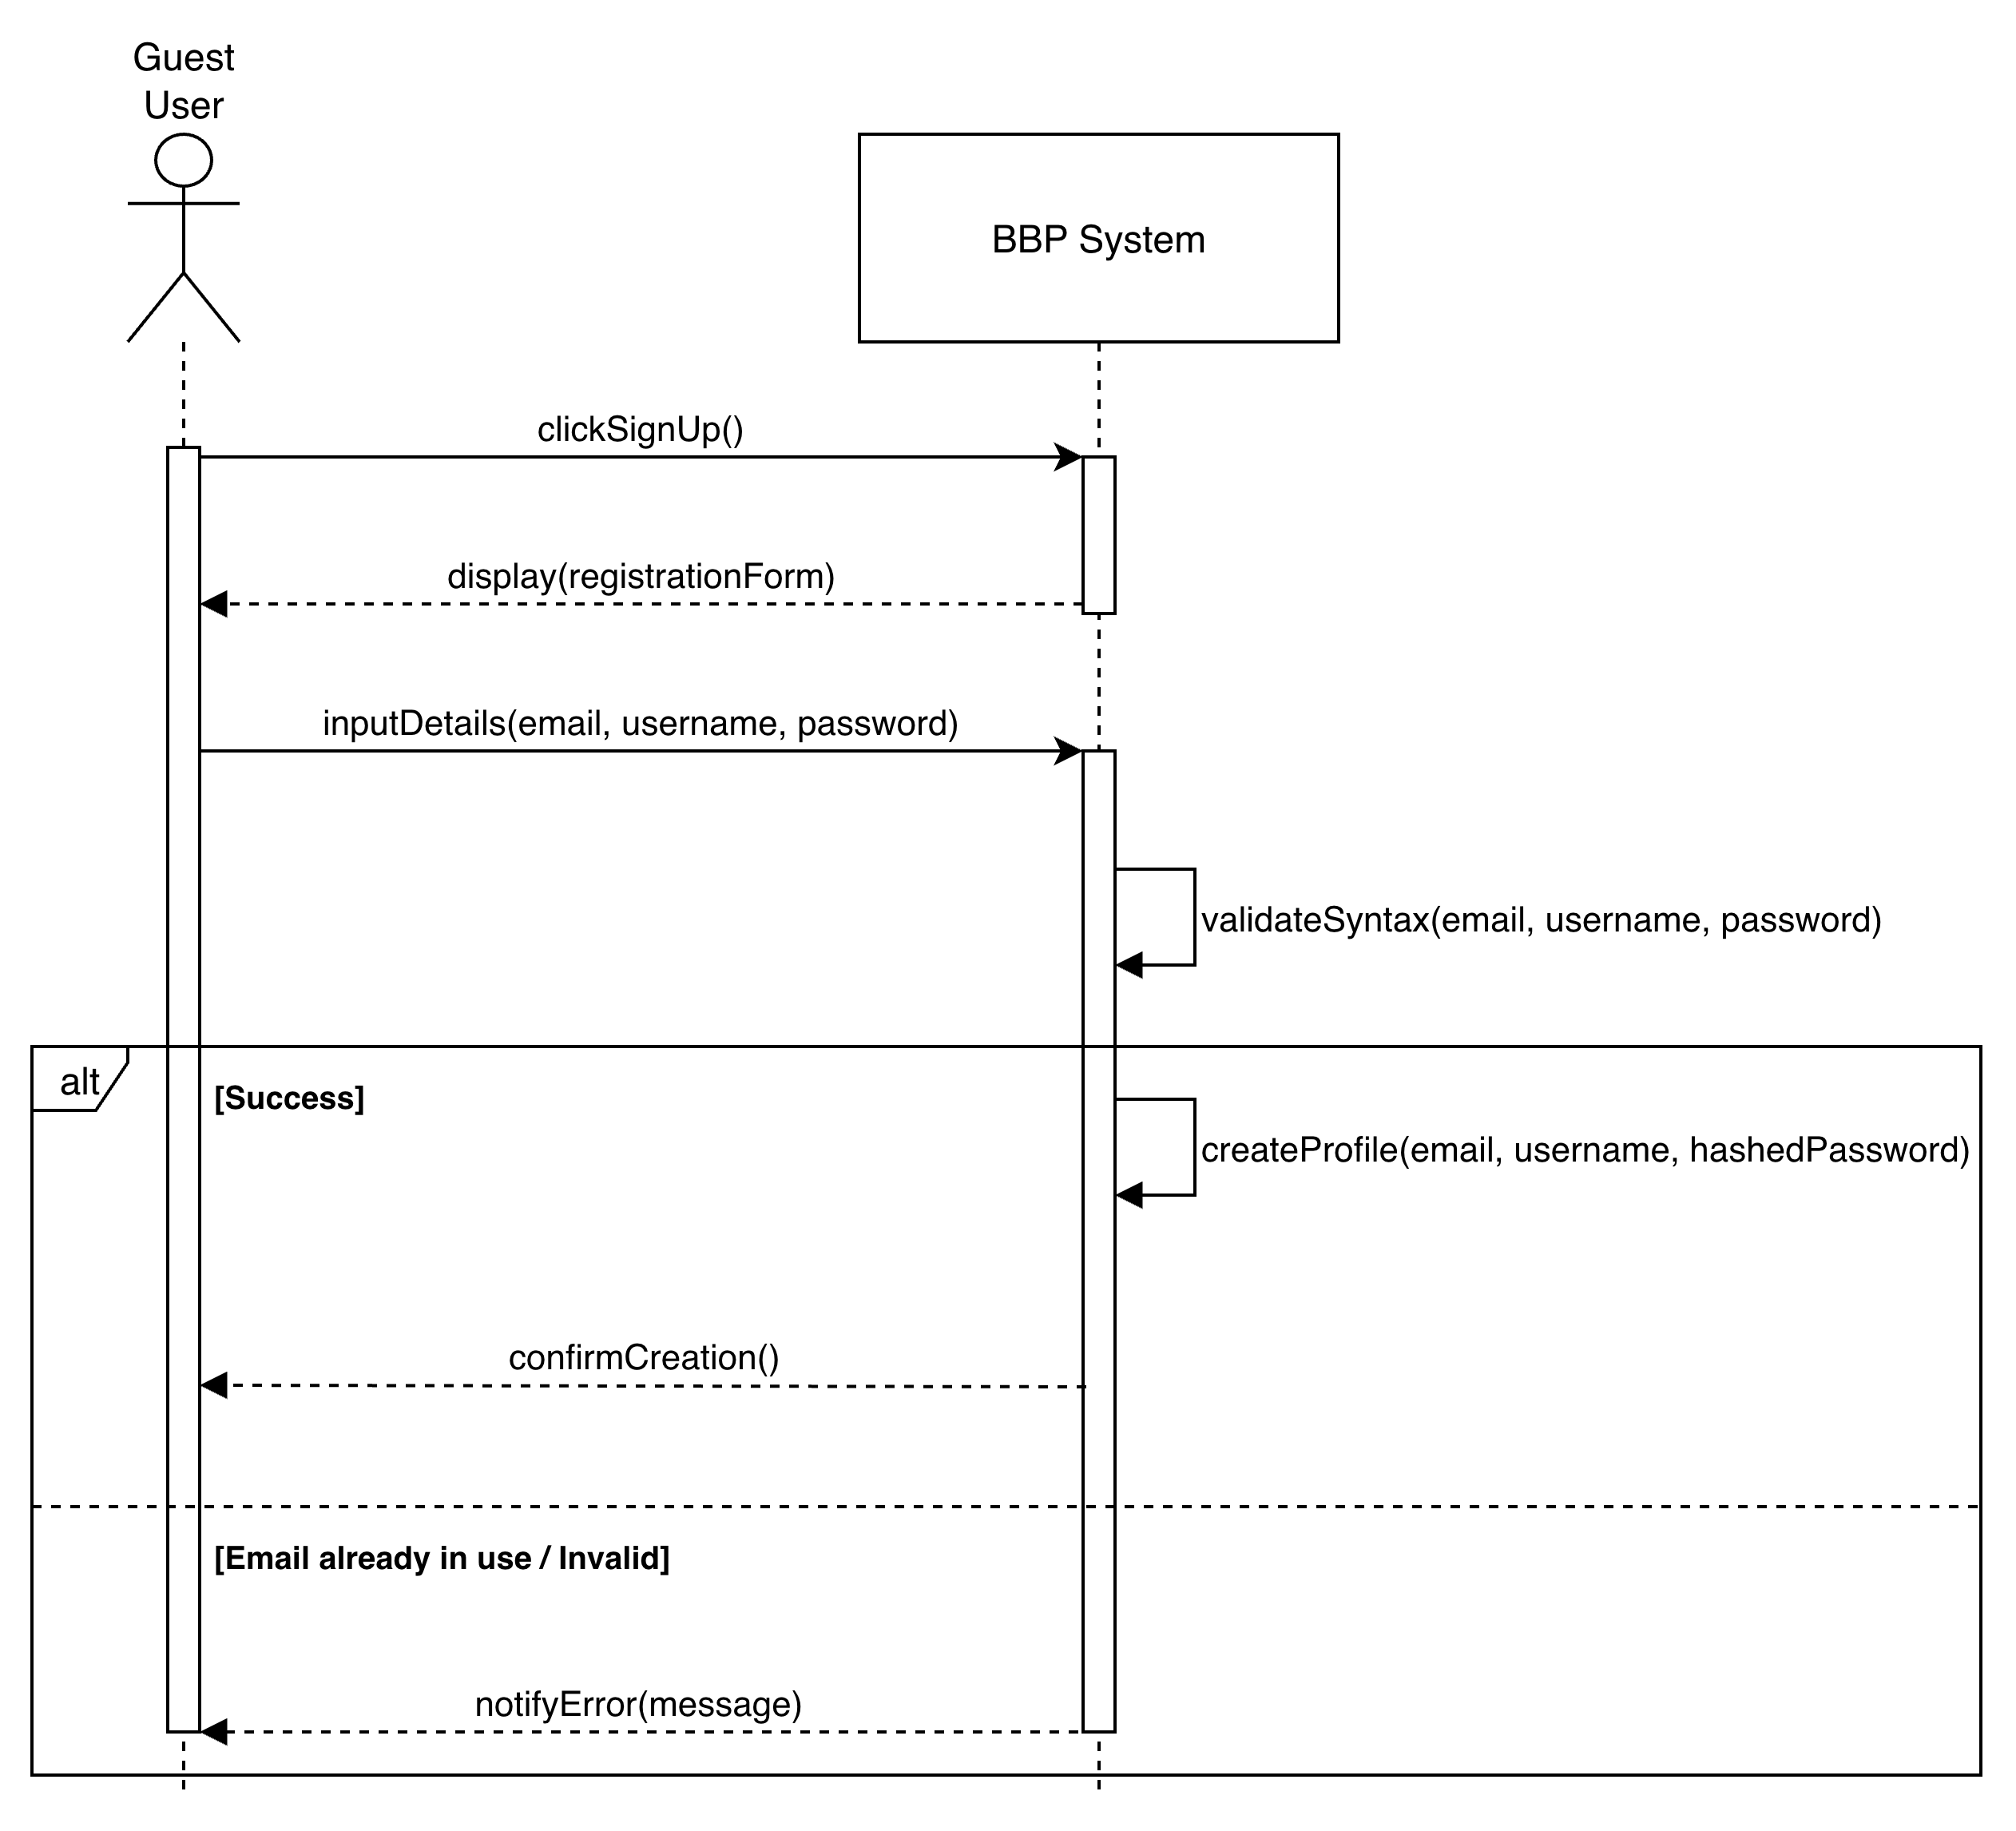
\includegraphics[width=\textwidth]{diagrams/sequence diagrams/uc1.png}
    \caption{Sequence Diagram for UC1: Sign Up}
    \label{fig:uc1_sequence}
\end{figure}

\begin{table}[H]
\centering
\begin{tabularx}{\textwidth}{|l|X|}
\hline
\multicolumn{2}{|c|}{\textbf{[UC2] - Log In}} \\ \hline
\textbf{Participating Actors} & \texttt{Registered User} \\ \hline
\textbf{Entry condition}      & The \texttt{Registered User} is not currently authenticated. \\ \hline
\textbf{Flow of events}       & 
\begin{enumerate}
    \item The \texttt{Registered User} clicks on "login".
    \item \texttt{BBP} displays the login form.
    \item The user inputs their credentials (\texttt{email}/\texttt{username}, \texttt{password}).
    \item The user clicks the "login" button.
    \item \texttt{BBP} hashes the \texttt{password} and validates it against the database.
    \item \texttt{BBP} retrieves the user's profile and starts a session.
    \item \texttt{BBP} redirects the user to the Home Page.
\end{enumerate} \\ \hline
\textbf{Exit conditions}      & The user is authenticated and can access restricted features. \\ \hline
\textbf{Exceptions}           & \textbf{Invalid Credentials:} \texttt{BBP} displays an error message and invites the user to retry. \\ \hline
\end{tabularx}
\caption{Use Case 2: Log In}
\label{tab:uc2}
\end{table}

\begin{figure}[H]
    \centering
    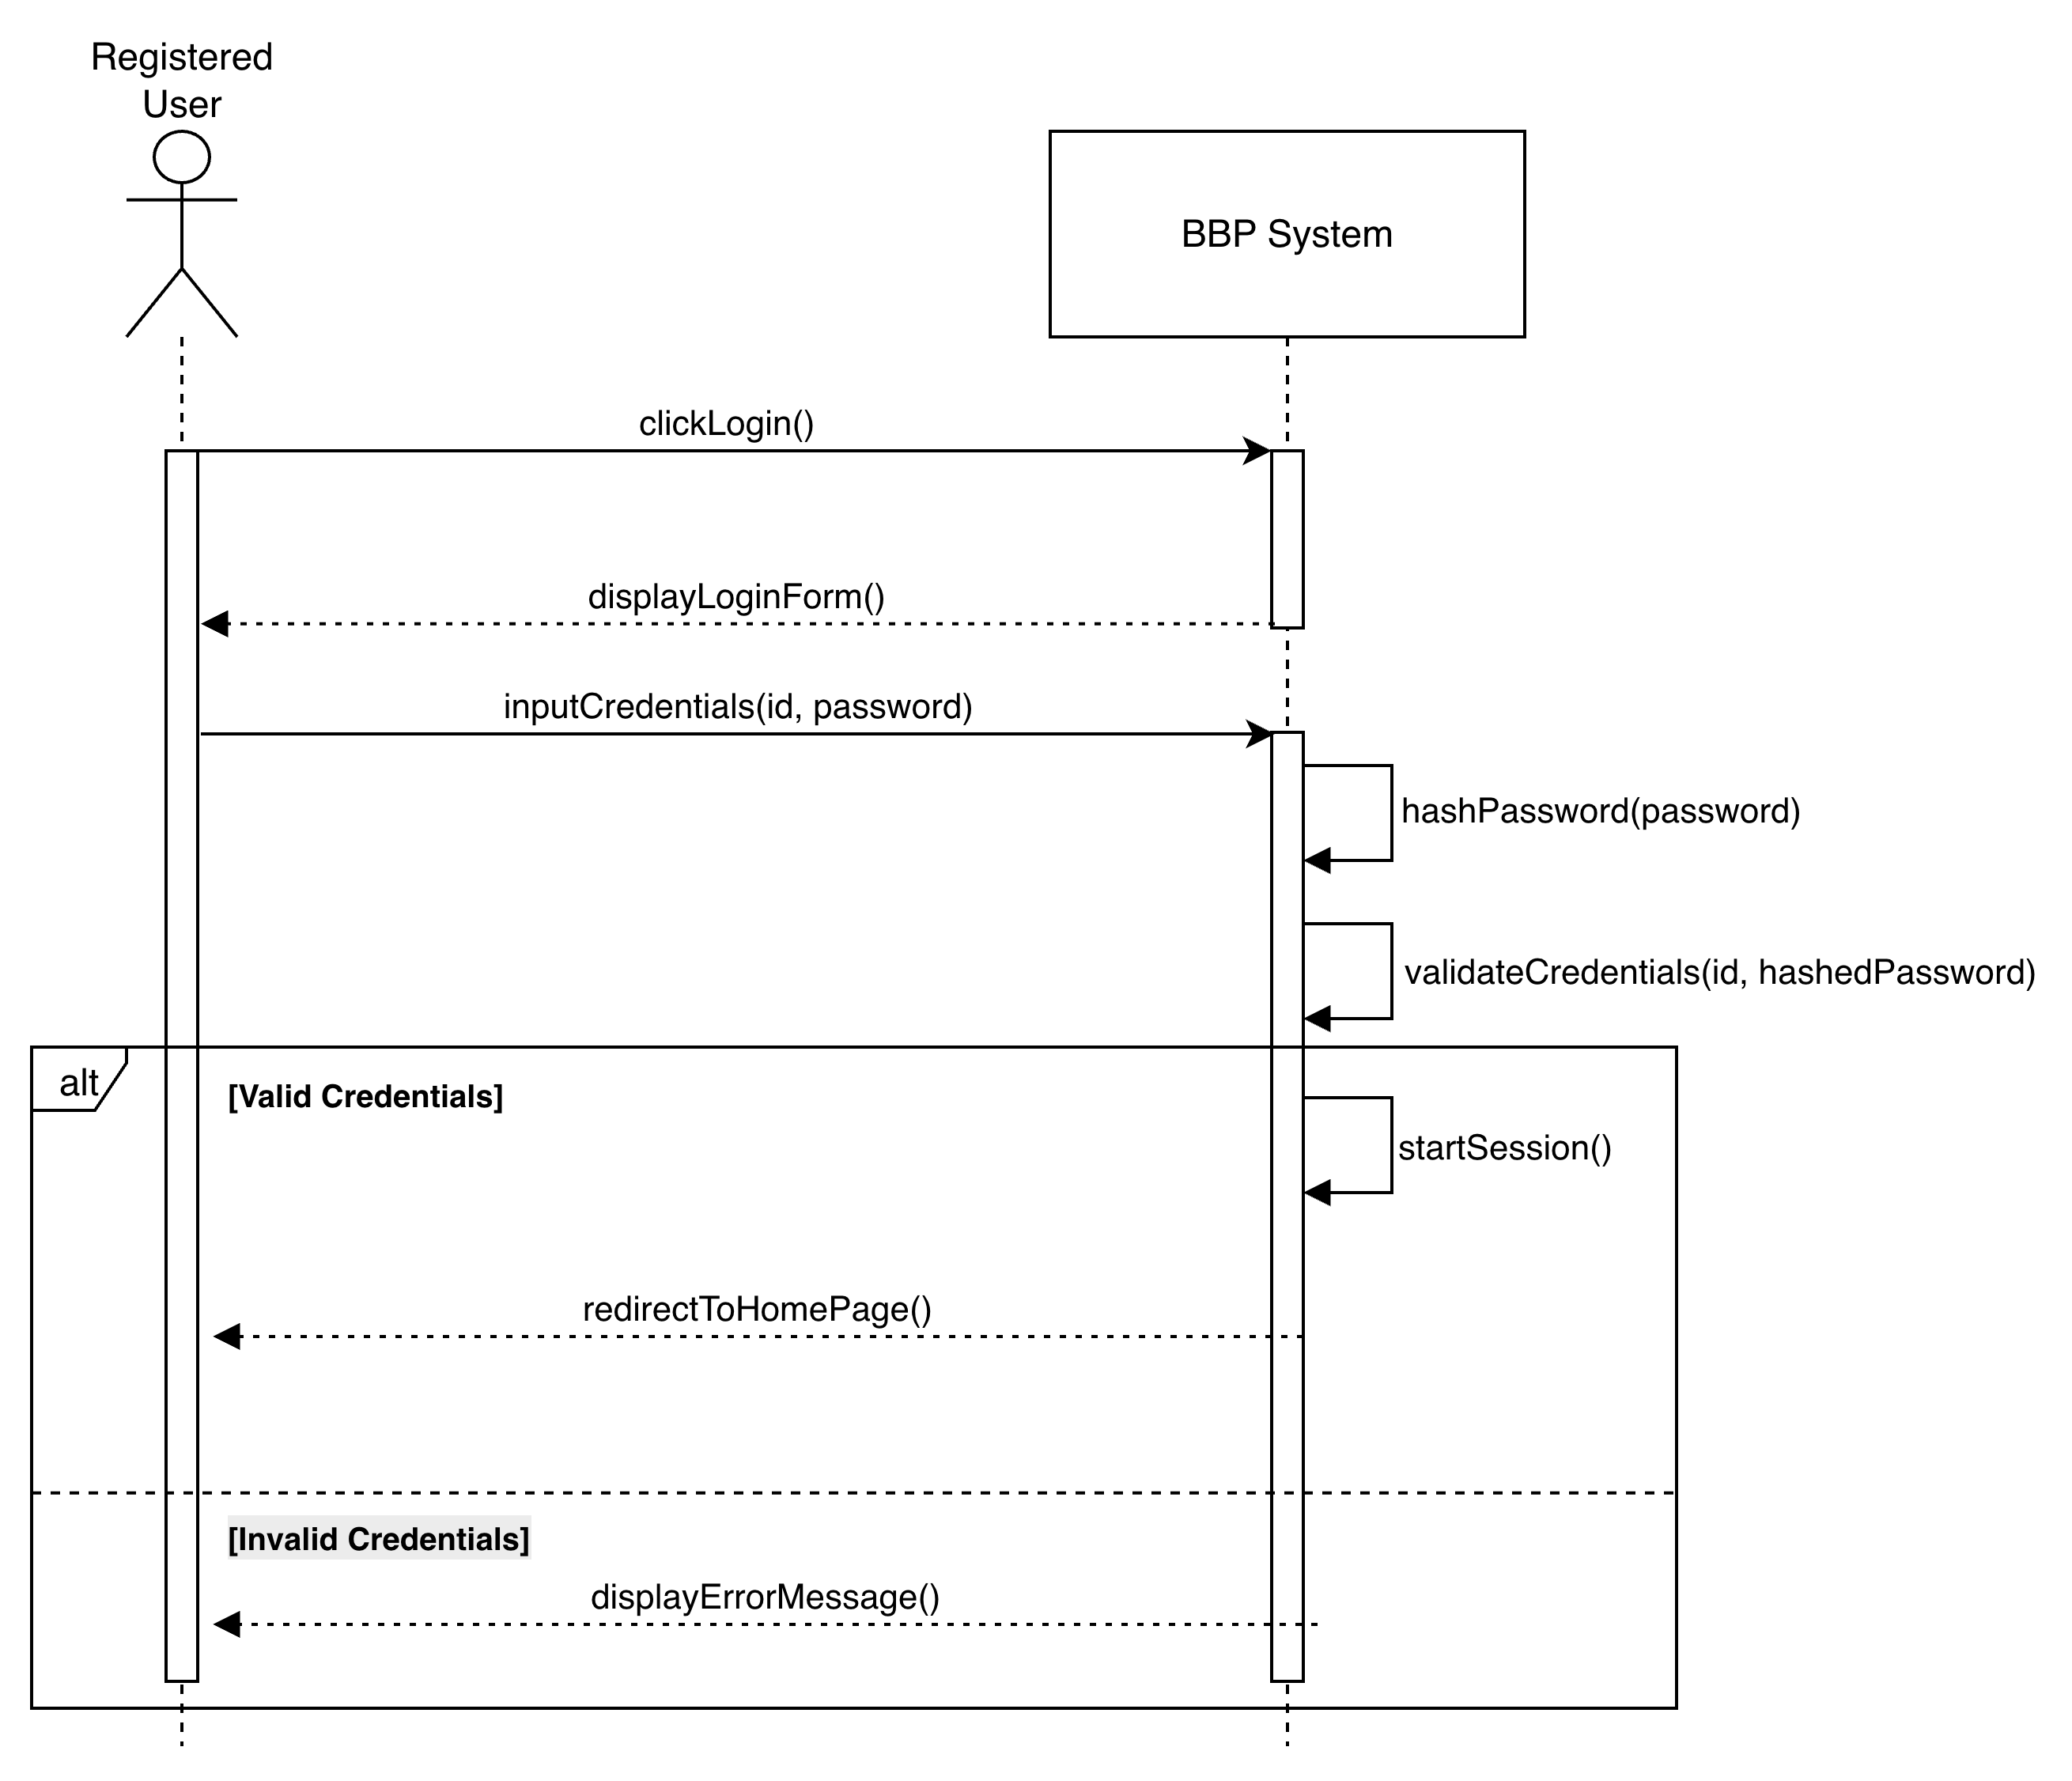
\includegraphics[width=\textwidth]{diagrams/sequence diagrams/uc2.png}
    \caption{Sequence Diagram for UC2: Log In}
    \label{fig:uc2_sequence}
\end{figure}

\begin{table}[H]
\centering
\begin{tabularx}{\textwidth}{|l|X|}
\hline
\multicolumn{2}{|c|}{\textbf{[UC3] - Record Trip Automatically}} \\ \hline
\textbf{Participating Actors} & \texttt{Registered User}, \texttt{Mobile Sensors}, \texttt{Weather Service} \\ \hline
\textbf{Entry condition}      & The \texttt{Registered User} is ready to automatically record his biking activity. \\ \hline
\textbf{Flow of events}       & 
\begin{enumerate}
    \item The \texttt{Registered User} clicks on "Start automatic recording".
    \item \texttt{BBP} enters detection mode and starts monitoring \texttt{GPS speed}.
    \item \texttt{BBP} detects biking activity (\texttt{speed} > \texttt{threshold}).
    \item \texttt{BBP} starts the recording session.
    \item \texttt{BBP} continuously logs \texttt{GPS coordinates} and \texttt{timestamps} (\texttt{trajectory}).
    \item \texttt{BBP} monitors \texttt{accelerometer}/\texttt{gyroscope} for anomalies (e.g., potholes).
    \item The user presses "End Automatic Record" button.
    \item \texttt{BBP} stores the detailed raw data (\texttt{GPS}, \texttt{trajectory}, \texttt{timestamps}).
    \item \texttt{BBP} retrieves historical meteorological data from the \texttt{Weather Service} and links it with the trip.
    \item \texttt{BBP} analyzes \texttt{sensors} data to identify potholes and stores them as \texttt{PENDING}.
    \item \texttt{BBP} calculates the specific statistics (\texttt{total distance}, \texttt{average speed}, and \texttt{duration}) and stores them.
    \item \texttt{BBP} saves the trip locally.
    \item \texttt{BBP} synchronizes the trip with the server.
\end{enumerate} \\ \hline
\textbf{Alternative Flows}    & 
\textbf{\texttt{Alternative 1}: Automatic Pause and Resume} \newline
1. If \texttt{speed} drops below \texttt{threshold} during Step 5, \texttt{BBP} pauses data acquisition. \newline
2. \texttt{BBP} continues monitoring \texttt{GPS speed} in the background. \newline
3. When \texttt{speed} exceeds \texttt{threshold} again, \texttt{BBP} resumes the recording session and returns to Step 5. \\ \hline
\textbf{Exit conditions}      & A new trip is recorded with its potholes, statistics, and weather conditions. \\ \hline
\textbf{Exceptions} & None. \\ \hline

\end{tabularx}
\caption{Use Case 3: Record Trip Automatically}
\label{tab:uc3}
\end{table}

\begin{figure}[H]
    \centering
     
\includegraphics[width=\textwidth]{diagrams/sequence diagrams/uc3.png}
    \caption{Sequence Diagram for UC3: Record Trip Automatically}
    \label{fig:uc3_sequence}
\end{figure}

\begin{table}[H]
\centering
\begin{tabularx}{\textwidth}{|l|X|}
\hline
\multicolumn{2}{|c|}{\textbf{[UC4] - Record Trip Manually}} \\ \hline
\textbf{Participating Actors} & \texttt{Registered User}, \texttt{Map Service} \\ \hline
\textbf{Entry condition}      & The \texttt{Registered User} is ready to manually insert trip information. \\ \hline
\textbf{Flow of events}       & 
\begin{enumerate}
    \item The user selects "Manual Record".
    \item \texttt{BBP} presents a form to insert trip details.
    \item \textbf{Loop} for adding streets to the trip:
    \begin{enumerate}
        \item The user specifies a street name.
        \item \texttt{BBP} queries the \texttt{Map Service} with the provided street name.
        \item \texttt{BBP} displays the found streets to the user.
        \item The user selects one of the found streets.
        \item The user selects a \texttt{path status} for the street: \texttt{OPTIMAL}, \texttt{MEDIUM}, \texttt{SUFFICIENT}, \texttt{REQUIRES\_MAINTENANCE}, or \texttt{PERMANENTLY\_CLOSE}.
        \item \texttt{BBP} adds the chosen street and its associated status to the trip entry.
    \end{enumerate}
    \item The user submits the form.
    \item \texttt{BBP} queries the \texttt{Map Service} to retrieve the \texttt{GPS coordinates} for each selected street.
    \item \texttt{BBP} identifies the intersections between each pair of sequential streets.
    \item \texttt{BBP} computes the \texttt{total distance} of the path.
    \item \texttt{BBP} confirms the submission.
    \item \texttt{BBP} saves the data.
\end{enumerate} \\ \hline
\textbf{Exit conditions}      & A new manual trip is recorded, including calculated \texttt{total distance} and street-specific statuses. \\ \hline
\textbf{Exceptions}           & 
\textbf{Invalid Location:} The system cannot identify the street provided; operation aborted. \newline
\textbf{Map Service Unavailable:} \texttt{BBP} shows an error and cancels the operation. \\ \hline
\end{tabularx}
\caption{Use Case 4: Record Trip Manually}
\label{tab:uc4}
\end{table}

\begin{figure}[H]
    \centering
    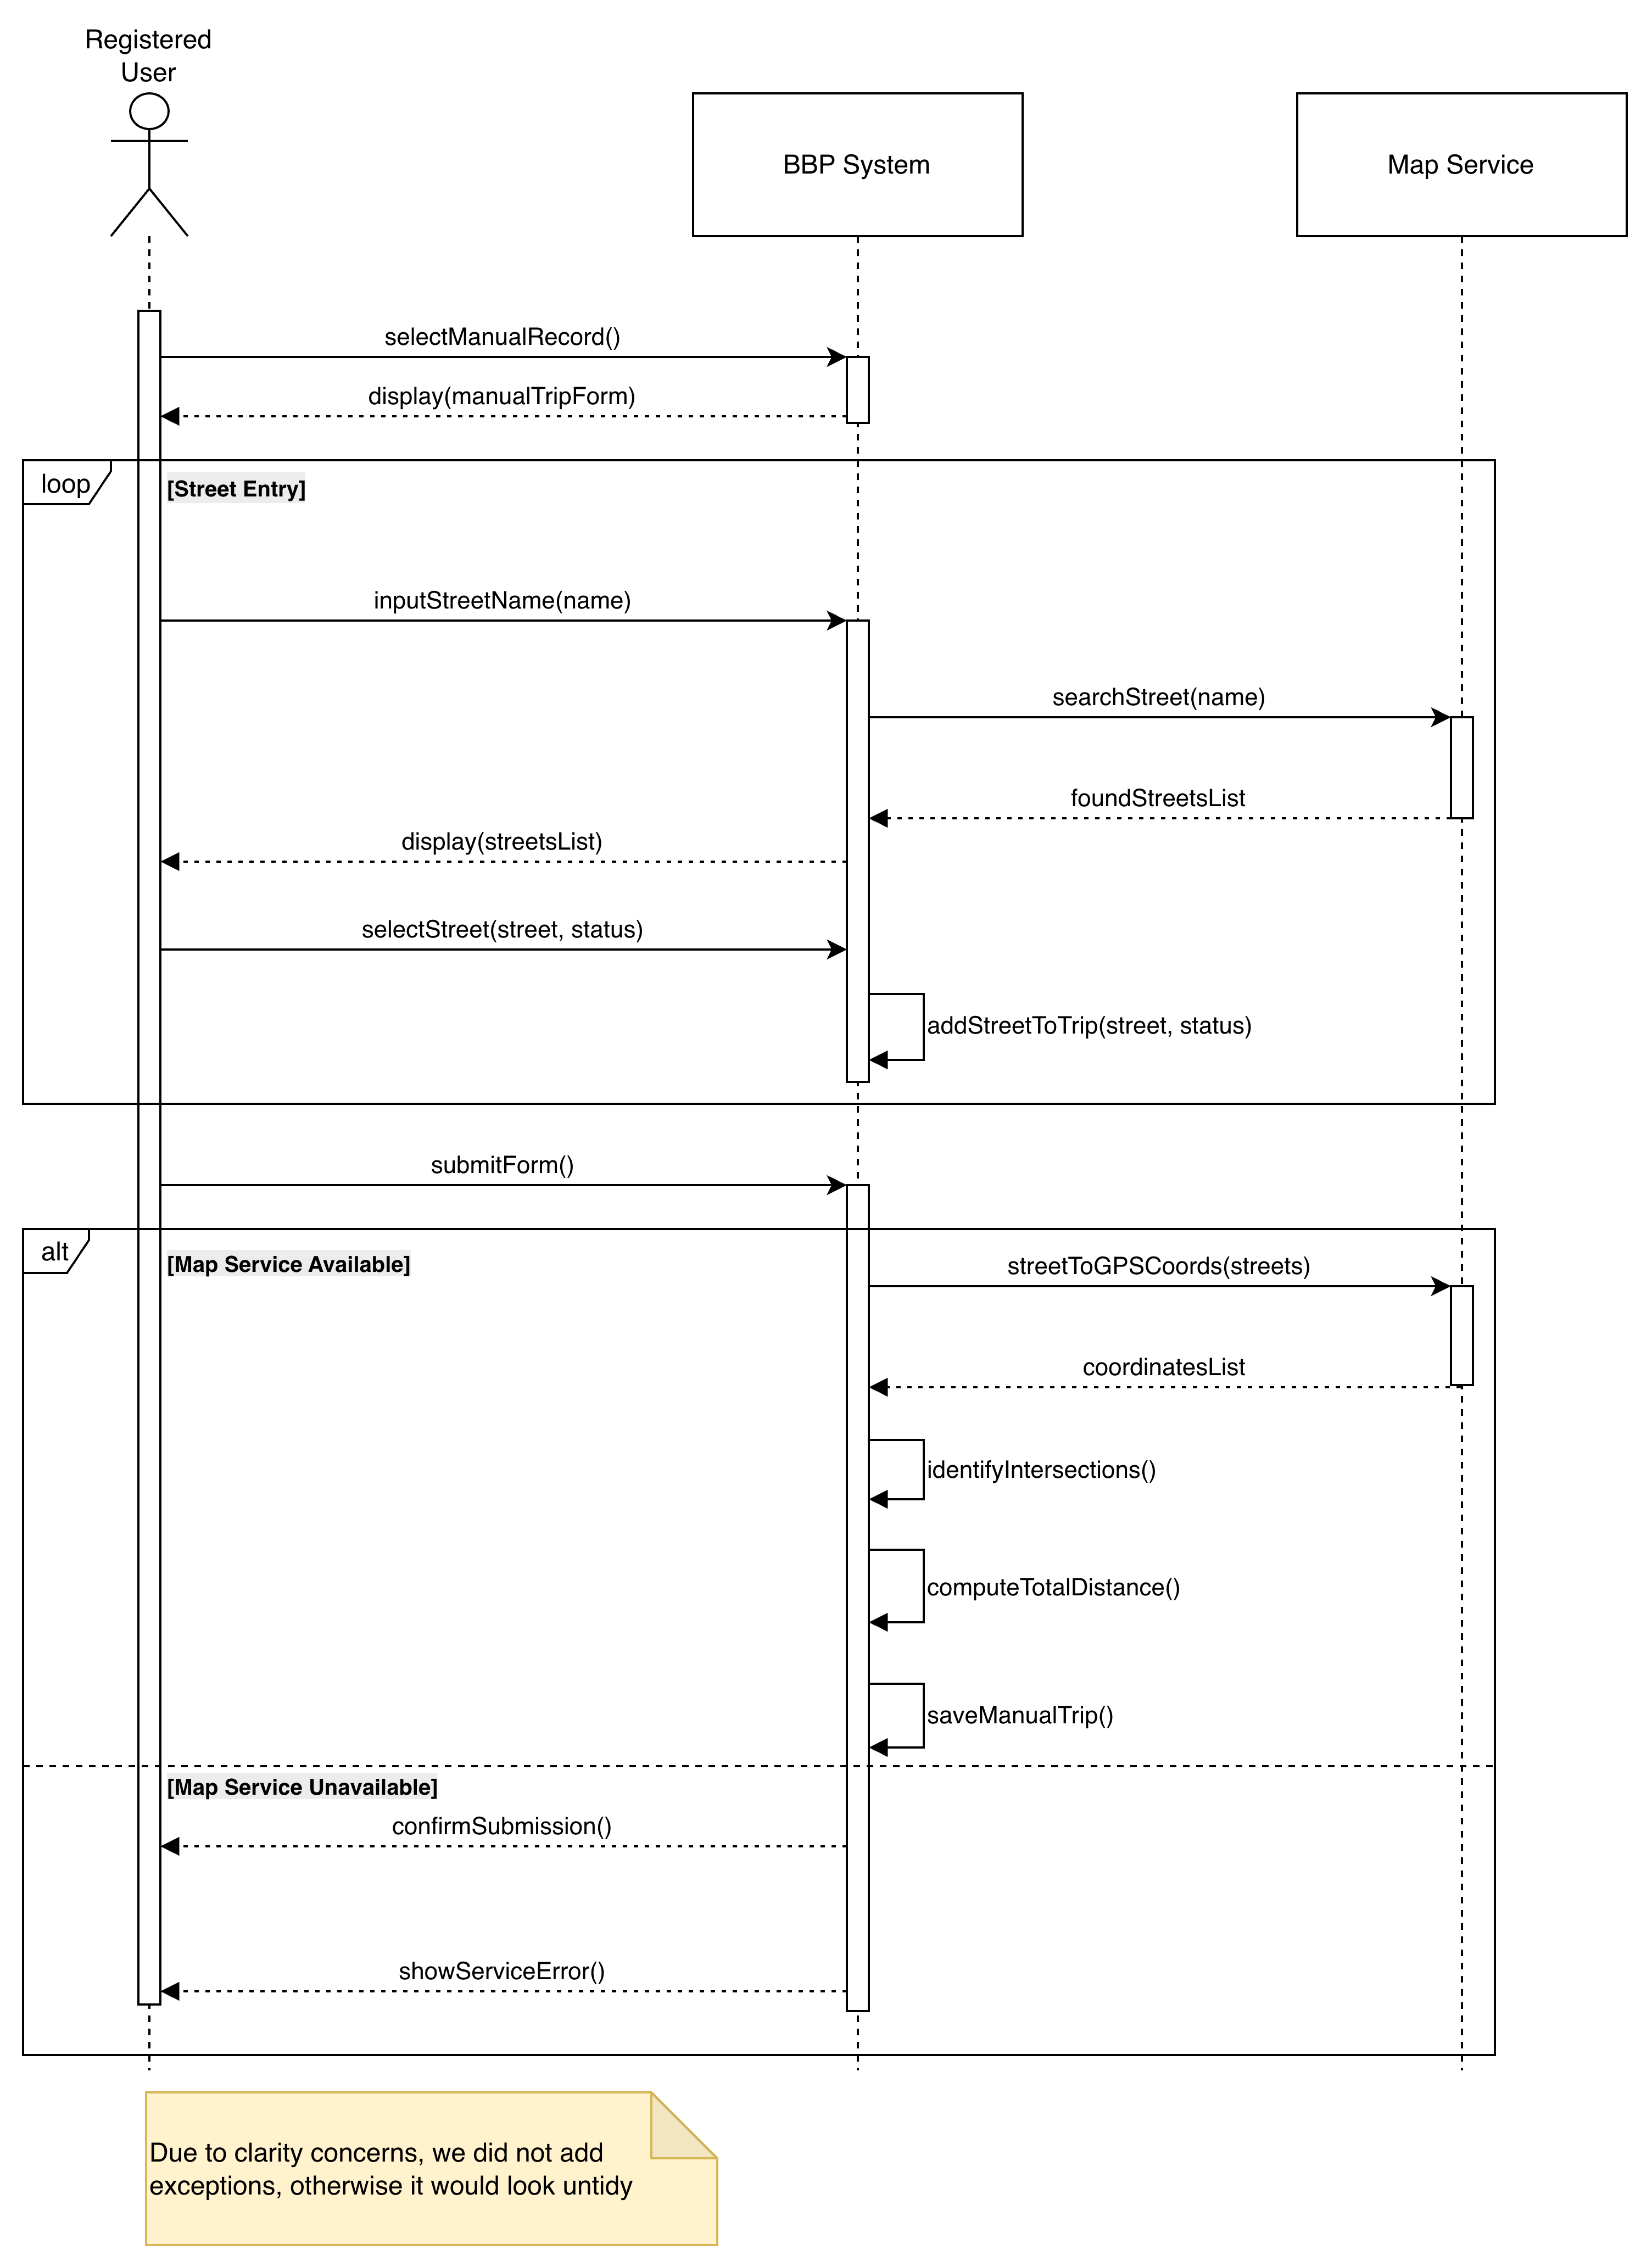
\includegraphics[width=\textwidth]{diagrams/sequence diagrams/uc4.png}
    \caption{Sequence Diagram for UC4: Record Trip Manually}
    \label{fig:uc4_sequence}
\end{figure}

\begin{table}[H]
\centering
\begin{tabularx}{\textwidth}{|l|X|}
\hline
\multicolumn{2}{|c|}{\textbf{[UC5] - Validate Obstacle}} \\ \hline
\textbf{Participating Actors} & \texttt{Registered User}, \texttt{Map Service} \\ \hline
\textbf{Entry condition}      & The \texttt{Registered User} is on their personal history page and is ready to validate an automatically recorded trip. \\ \hline
\textbf{Flow of events}       & 
\begin{enumerate}
    \item The \texttt{Registered User} chooses one of their automatically recorded private trips.
    \item \texttt{BBP} highlights potential anomalies of the selected trip on the map interface.
    \item The user clicks the "Start Validating" button.
    \item \textbf{Loop} for each identified \texttt{}{PENDING} anomaly:
    \begin{enumerate}
        \item \texttt{BBP} displays the details and location of a specific anomaly.
        \item The user reviews the anomaly.
        \item The user chooses a validation action: \texttt{Alternative 1} or \texttt{Alternative 2}.
    \end{enumerate}
    \item \texttt{BBP} displays a summary of the validation results for all reviewed anomalies.
    \item \texttt{BBP} prompts the user to select a \texttt{ status} for the trip.
    \item The user selects the \texttt{status} from: \texttt{OPTIMAL}, \texttt{MEDIUM}, \texttt{SUFFICIENT}, \texttt{REQUIRES\_MAINTENANCE}, or \texttt{PERMANENTLY\_CLOSE}.
    \item The user saves the validated trip.
    \item \texttt{BBP} updates the trip data in the database.
\end{enumerate} \\ \hline
\textbf{Alternative Flows}    & 
\textbf{\texttt{Alternative 1}: Confirm Detection} \newline
1. The user confirms the anomaly detection. \newline
2. \texttt{BBP} updates the pothole status to \texttt{CONFIRMED}. \newline
\textbf{\texttt{Alternative 2}: Reject Detection} \newline
1. The user rejects the anomaly detection. \newline
2. \texttt{BBP} updates the pothole status to \texttt{REJECTED}. \\ \hline
\textbf{Exit conditions}      & Trip obstacles are validated, a \texttt{path status} is assigned, and the trip is ready for optional publication. \\ \hline
\textbf{Exceptions}           & \textbf{Map Service Unavailable:} \texttt{BBP} shows an error regarding the map rendering and prompts the user to try the validation later. \\ \hline
\end{tabularx}
\caption{Use Case 5: Validate Obstacle}
\label{tab:uc5}
\end{table}

\begin{figure}[H]
    \centering
    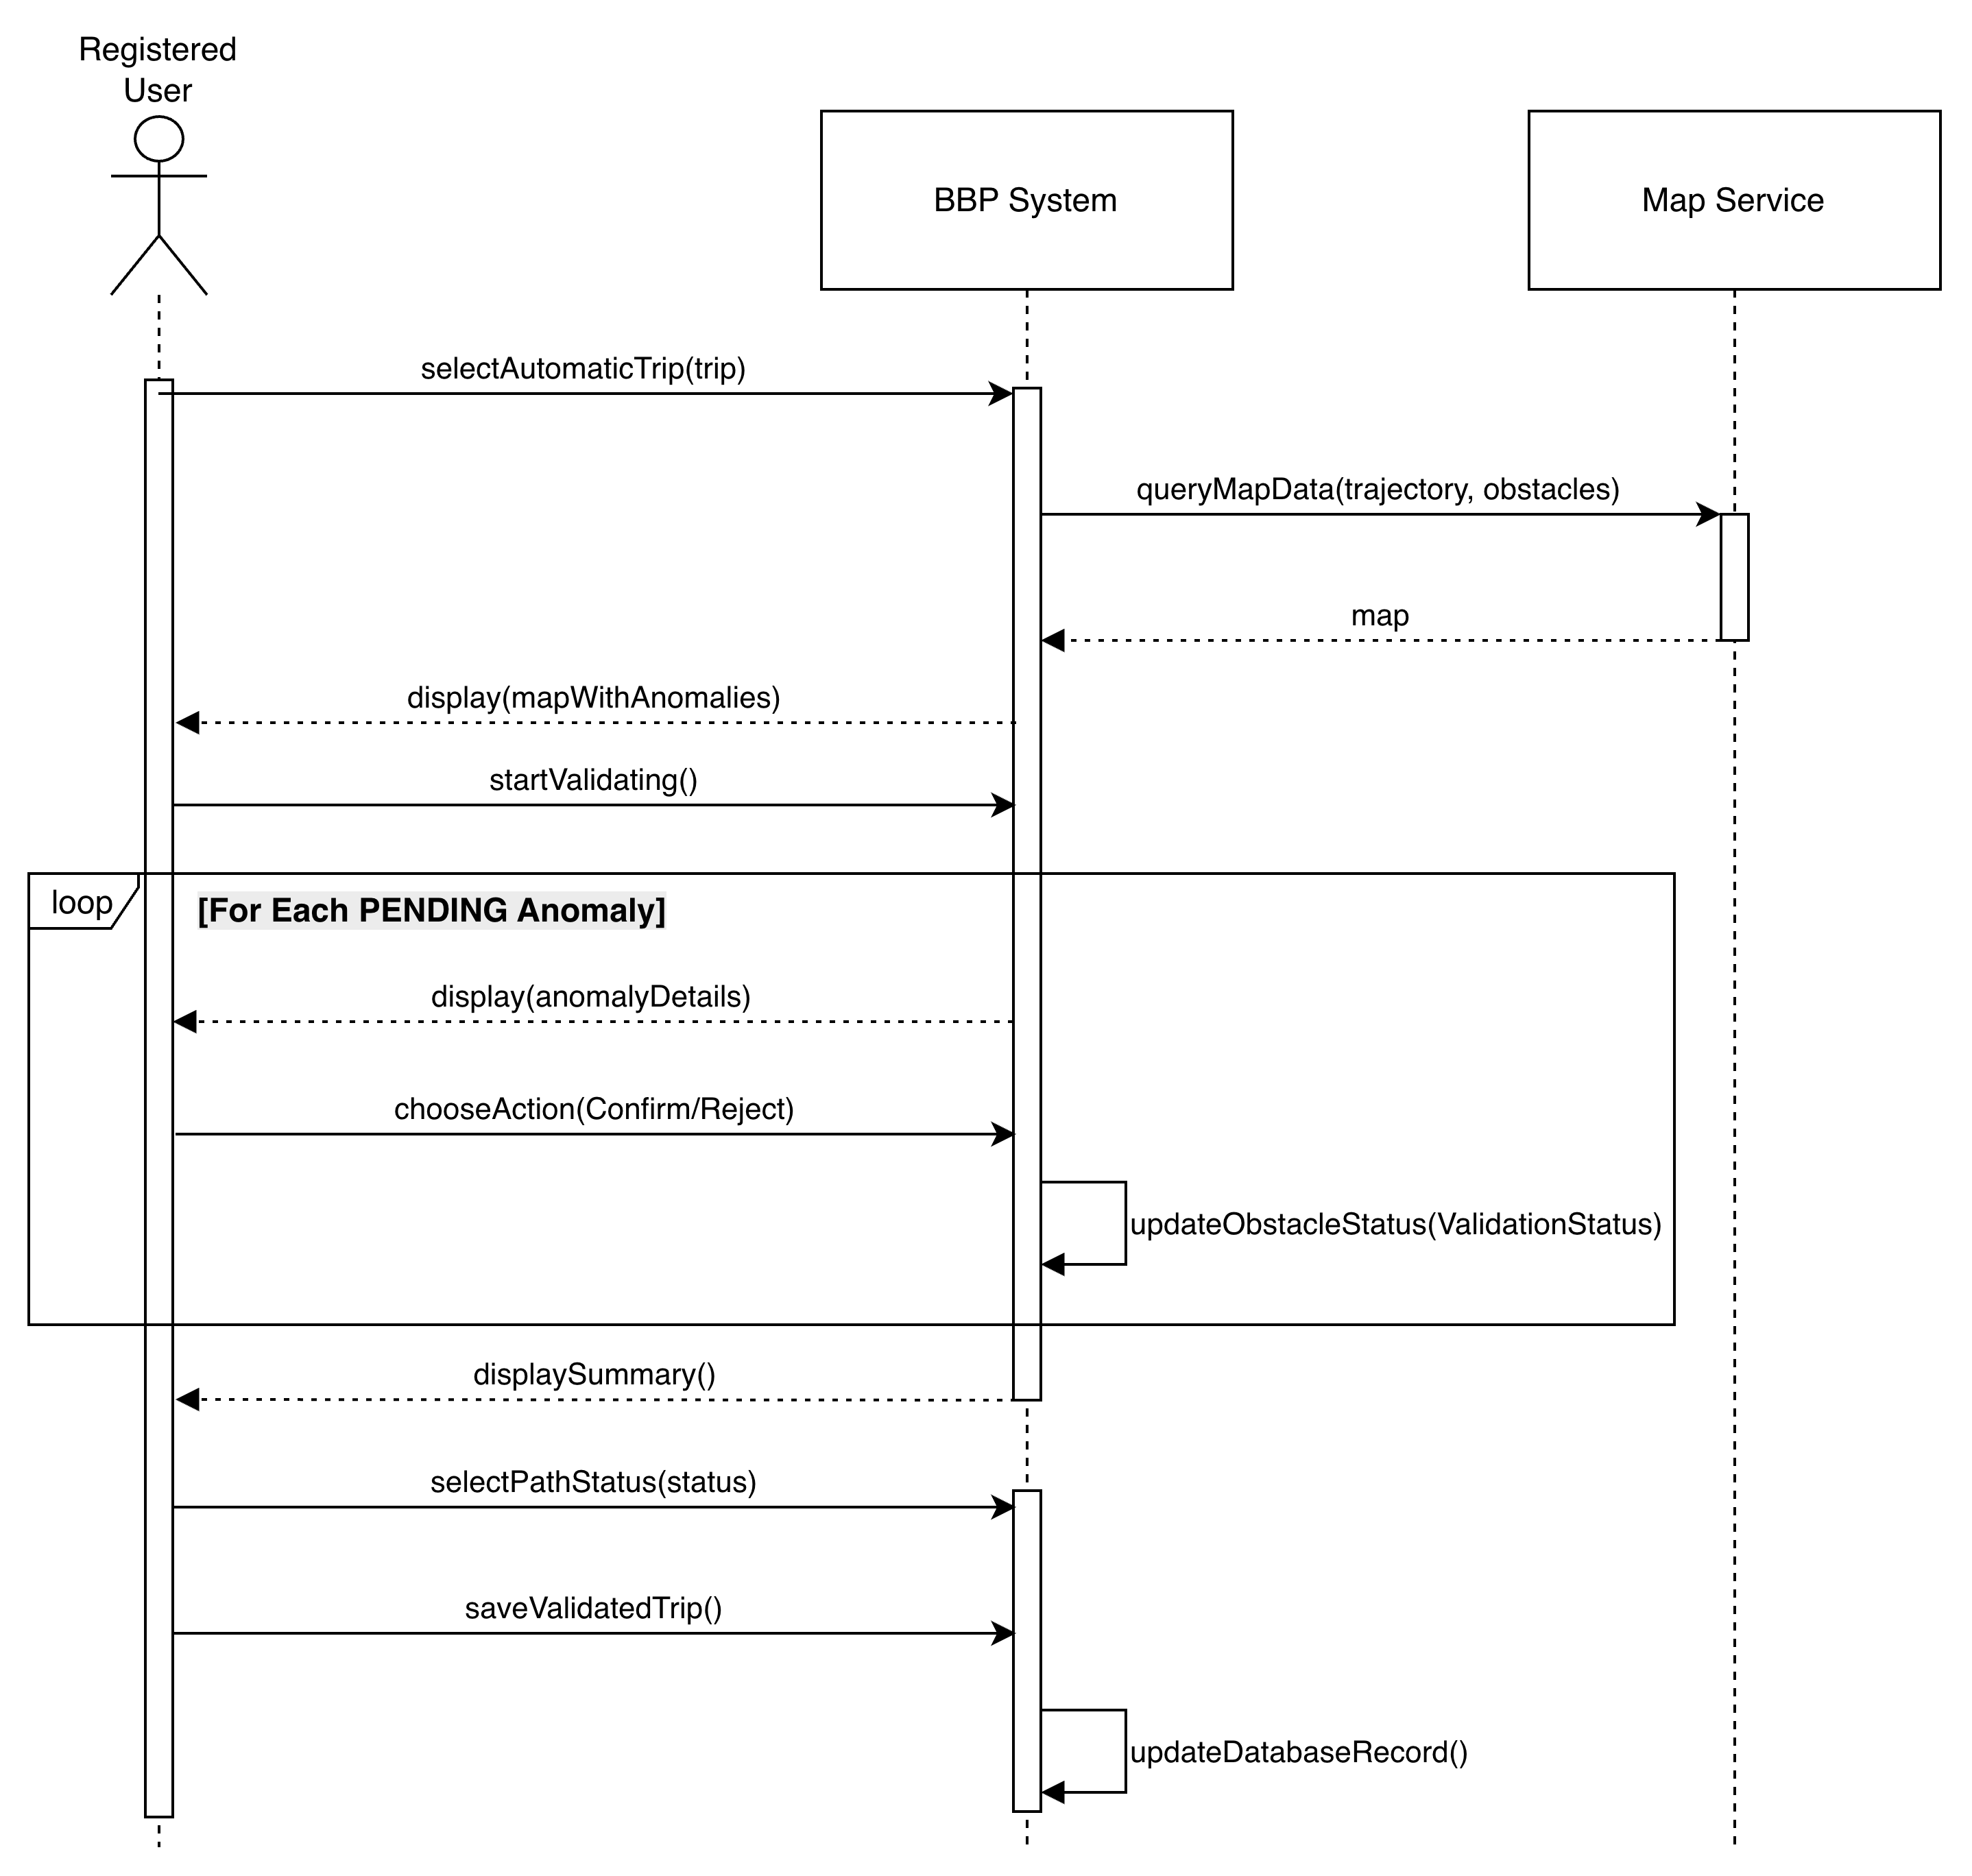
\includegraphics[width=\textwidth]{diagrams/sequence diagrams/uc5.png}
    \caption{Sequence Diagram for UC5: Validate Obstacle}
    \label{fig:uc5_sequence}
\end{figure}


\begin{table}[H]
\centering
\begin{tabularx}{\textwidth}{|l|X|}
\hline
\multicolumn{2}{|c|}{\textbf{[UC6] - Publish Trip}} \\ \hline
\textbf{Participating Actors} & \texttt{Registered User} \\ \hline
\textbf{Entry condition}      & The \texttt{Registered User} has at least one \texttt{private} trip ready to publish. \\ \hline
\textbf{Flow of events}       & 
\begin{enumerate}
    \item The \texttt{Registered User} clicks on "My Trips".
    \item BBP displays the list of the user trips recorded over time.
    \item The user selects a specific trip from their history list.
    \item BBP displays the trip and its details.
    \item The user clicks the "publish" button.
    \item \texttt{BBP} anonymizes the trip data to protect user privacy.
    \item \texttt{BBP} triggers the \texttt{Data Merging algorithm} to integrate anonymized data with existing datasets (considering freshness and confirmations).
    \item \texttt{BBP} updates the \texttt{path score, path status, obstacles} based on the new \texttt{Trip}.
    \item \texttt{BBP} confirms the successful publication to the user.
\end{enumerate} \\ \hline
\textbf{Exit conditions}      & Trip data has been integrated into the public path and is available to all users. \\ \hline
\textbf{Exceptions}           & None. \\ \hline
\end{tabularx}
\caption{Use Case 6: Publish Trip}
\label{tab:uc6}
\end{table}

\begin{figure}[H]
    \centering
    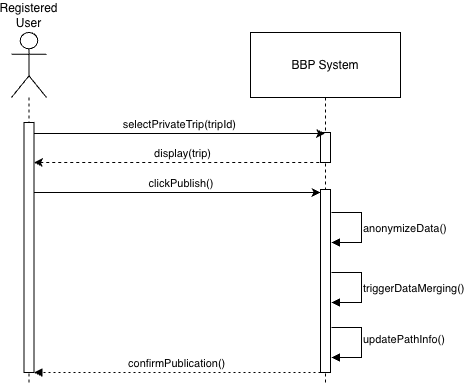
\includegraphics[width=\textwidth]{diagrams/sequence diagrams/uc6.png}
    \caption{Sequence Diagram for UC6: Publish Trip}
    \label{fig:uc6_sequence}
\end{figure}


\begin{table}[H]
\centering
\begin{tabularx}{\textwidth}{|l|X|}
\hline
\multicolumn{2}{|c|}{\textbf{[UC7] - View Private Trip}} \\ \hline
\textbf{Participating Actors} & \texttt{Registered User}, \texttt{Map Service} \\ \hline
\textbf{Entry condition}      & The \texttt{Registered User} has recorded at least one trip and wants to view it in detail. \\ \hline
\textbf{Flow of events}       & 
\begin{enumerate}
    \item The \texttt{Registered User} clicks on "My Trips".
    \item \texttt{BBP} displays the list of the user trips recorded over time.
    \item The user selects a specific trip from their history list.
    \item \texttt{BBP} queries the \texttt{Map Service} to fetch map data corresponding to the chosen trip's \texttt{GPS coordinates}.
    \item \texttt{BBP} displays a detailed view including the trip \texttt{trajectory} on the map, computed statistics, found/confirmed potholes, and the weather conditions recorded during the ride.
\end{enumerate} \\ \hline
\textbf{Exit conditions}      & The User successfully visualizes the detailed performance and environmental context of a single specific trip. \\ \hline
\textbf{Exceptions}           & \textbf{Map Service Unavailable:} \texttt{BBP} displays an error notification regarding the map interface but continues to display the statistics. \\ \hline
\end{tabularx}
\caption{Use Case 7: View Private Trip}
\label{tab:uc7}
\end{table}

\begin{figure}[H]
    \centering
    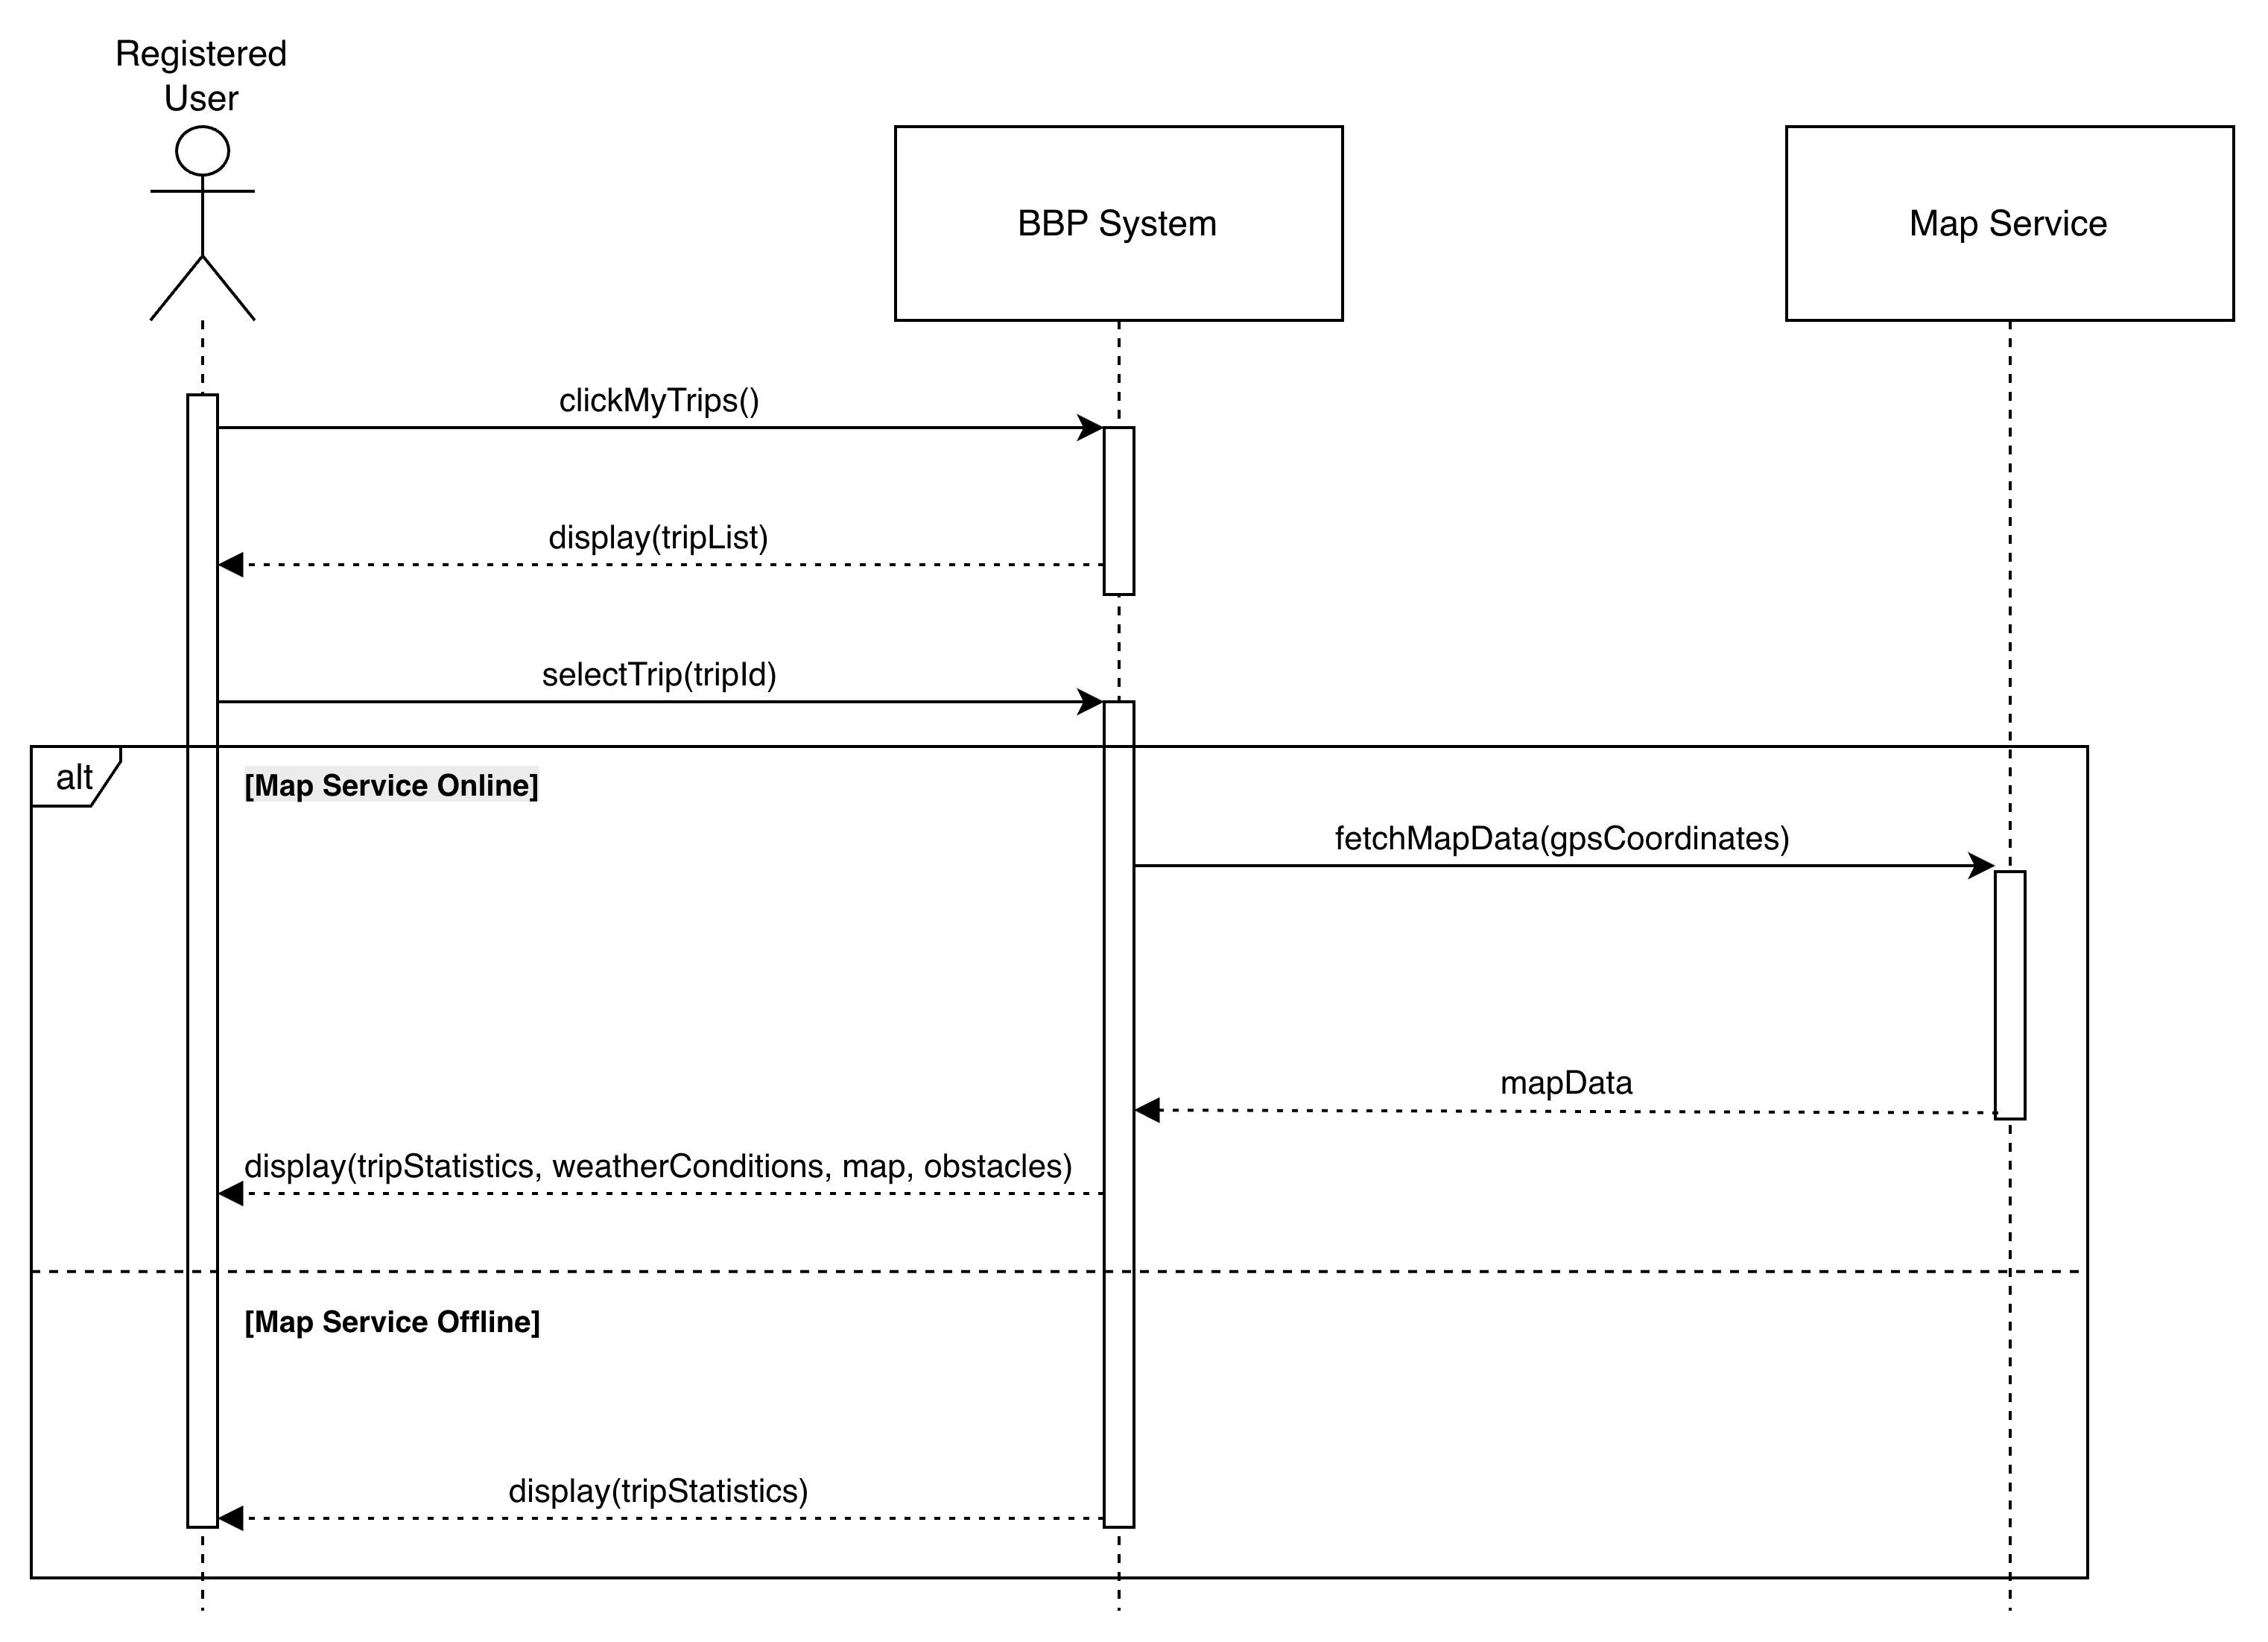
\includegraphics[width=\textwidth]{diagrams/sequence diagrams/uc7.png}
    \caption{Sequence Diagram for UC7: View Private Trip}
    \label{fig:uc7_sequence}
\end{figure}


\begin{table}[H]
\centering
\begin{tabularx}{\textwidth}{|l|X|}
\hline
\multicolumn{2}{|c|}{\textbf{[UC8] - Delete Private Trip}} \\ \hline
\textbf{Participating Actors} & \texttt{Registered User} \\ \hline
\textbf{Entry condition}      & The \texttt{Registered User} has recorded at least one trip and wants to delete it. \\ \hline
\textbf{Flow of events}       & 
\begin{enumerate}
    \item The \texttt{Registered User} clicks on "My Trips".
    \item \texttt{BBP} displays the list of the user trips recorded over time.
    \item The user long-presses on a specific trip from the history list.
    \item \texttt{BBP} displays an additional in-context menu.
    \item The user selects the "Delete" option.
    \item \texttt{BBP} displays a confirmation prompt.
    \item The user confirms the operation.
    \item \texttt{BBP} deletes the selected trip from the user history.
    \item \texttt{BBP} confirms the deletion.
\end{enumerate} \\ \hline
\textbf{Alternative Flows}    & 
\textbf{\texttt{Alternative 1}: user Cancels Deletion} \newline
1. At Step 7 of the \texttt{Flow of events}, the user cancels the operation. \newline
2. \texttt{BBP} aborts the deletion process. \newline
3. \texttt{BBP} returns the user to the history list without making changes. \\ \hline
\textbf{Exit conditions}      & The trip is removed from the \texttt{Registered user}'s private history. If previously published, the anonymized data remains in the aggregated \texttt{PATH} information. \\ \hline
\textbf{Exceptions} & None \\ \hline
\end{tabularx}
\caption{Use Case 8: Delete Private Trip}
\label{tab:uc8}
\end{table}

\begin{figure}[H]
    \centering
    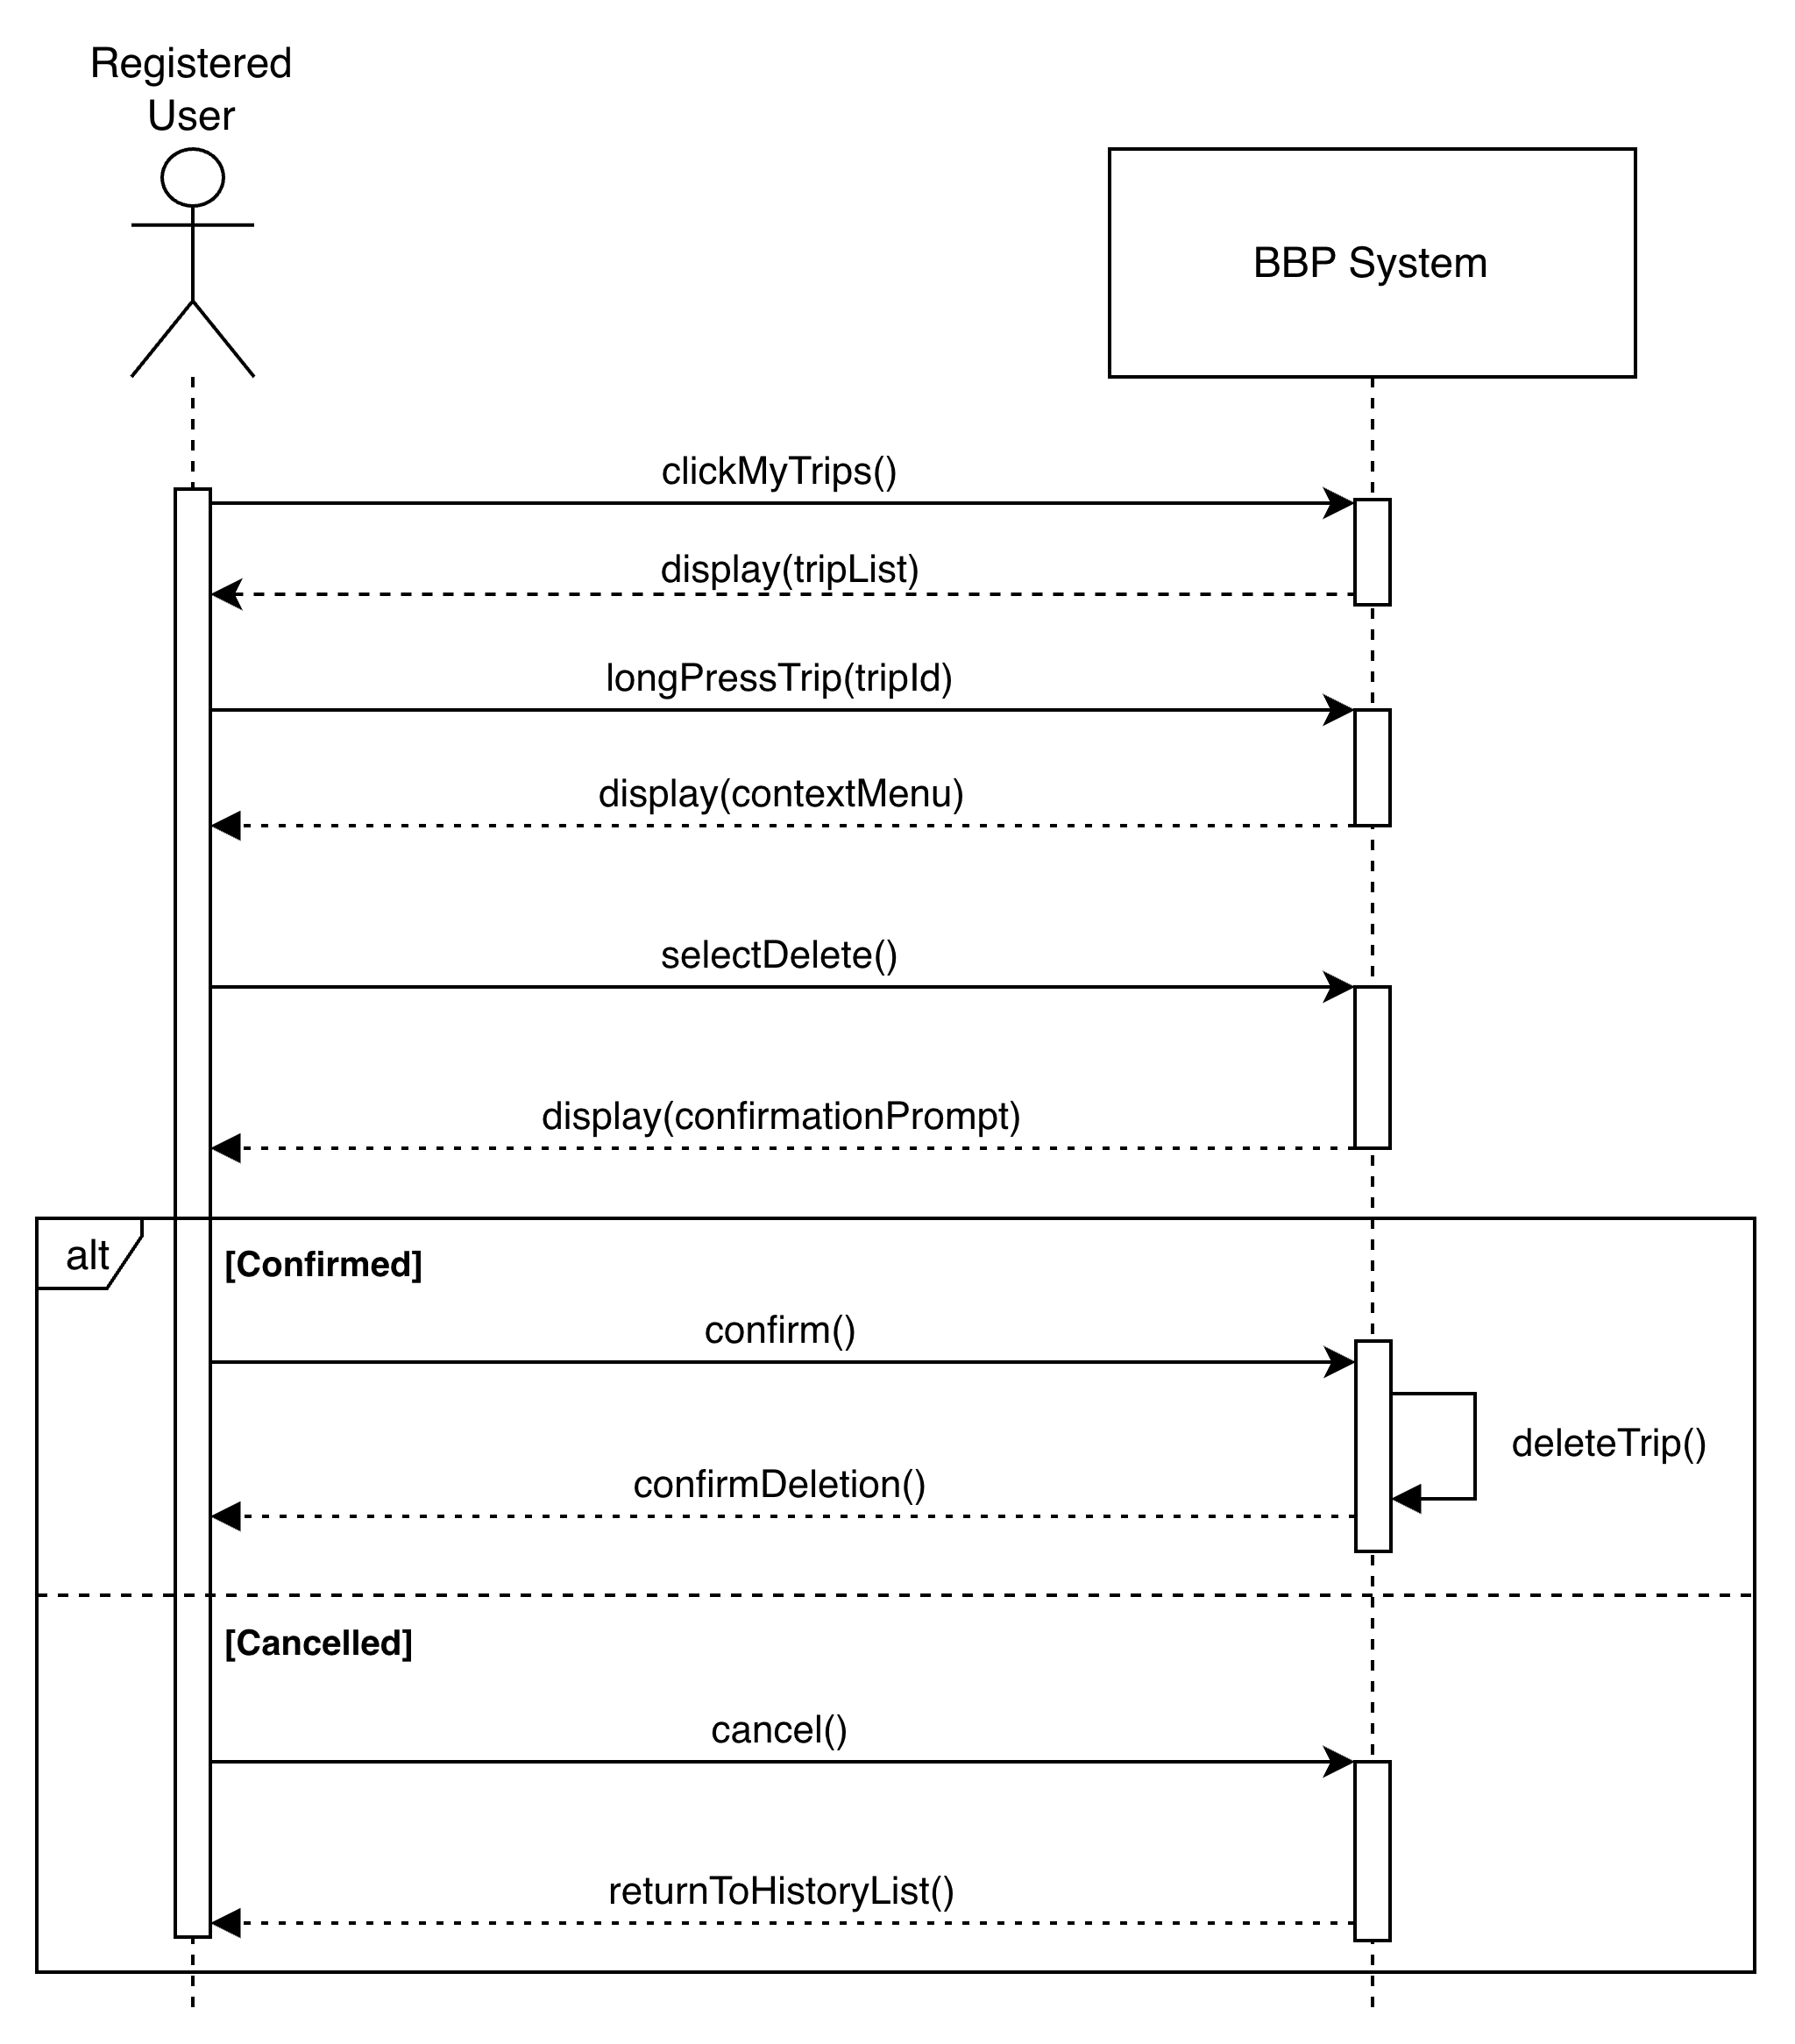
\includegraphics[width=\textwidth]{diagrams/sequence diagrams/uc8.png}
    \caption{Sequence Diagram for UC8: Delete Private Trip}
    \label{fig:uc8_sequence}
\end{figure}


\begin{table}[H]
\centering
\begin{tabularx}{\textwidth}{|l|X|}
\hline
\multicolumn{2}{|c|}{\textbf{[UC9] - SearchPath}} \\ \hline
\textbf{Participating Actors} & \texttt{User} , \texttt{Map Service} \\ \hline
\textbf{Entry condition}      & The \texttt{User} is ready to search paths between two points. \\ \hline
\textbf{Flow of events}       & 
\begin{enumerate}
    \item The user clicks on the search bar.
    \item \texttt{BBP} displays the search form with the map interface.
    \item The user chooses the input method: \texttt{Alternative 1} or \texttt{Alternative 2}.
    \item \texttt{BBP} searches for paths using the provided \texttt{Origin} and \texttt{Destination} endpoints.
    \item \texttt{BBP} ranks the found paths by the previously computed/updated score.
    \item \texttt{BBP} shows the ranked list of paths to the user.
\end{enumerate} \\ \hline
\textbf{Alternative Flows}    & 
\textbf{\texttt{Alternative 1}: Text Search}
\begin{enumerate}
    \item \textbf{Loop} for \texttt{Origin} and \texttt{Destination} endpoints:
    \begin{enumerate}
        \item The user enters an endpoint street name.
        \item \texttt{BBP} queries the \texttt{Map Service} with the provided street name.
        \item \texttt{BBP} displays the found streets to the user.
        \item The user selects one of the found streets.
        \item \texttt{BBP} saves the selection as the endpoint value.
    \end{enumerate}
\end{enumerate}
\textbf{\texttt{Alternative 2}: Map Selection}
\begin{enumerate}
    \item \textbf{Loop} for \texttt{Origin} and \texttt{Destination} endpoints:
    \begin{enumerate}
        \item The user clicks/taps on a point on the map.
        \item \texttt{BBP} queries the \texttt{Map Service} to identify the location.
        \item \texttt{BBP} displays the address/location of the selected point.
        \item The user confirms the selection.
        \item \texttt{BBP} saves the selection as the endpoint value.
    \end{enumerate}
\end{enumerate} \\ \hline
\textbf{Exit conditions}      & User is shown available paths ready to be viewed in details. \\ \hline
\textbf{Exceptions}           & 
\textbf{Invalid Location:} The system cannot identify the point; operation aborted. \newline
\textbf{Map Service Unavailable:} \texttt{BBP} shows an error and suggests trying again later. \newline
\textbf{No Paths Found:} \texttt{BBP} displays a "Path not found" message. \\ \hline
\end{tabularx}
\caption{Use Case 9: Search Path}
\label{tab:uc9}
\end{table}

\begin{figure}[H]
    \centering
    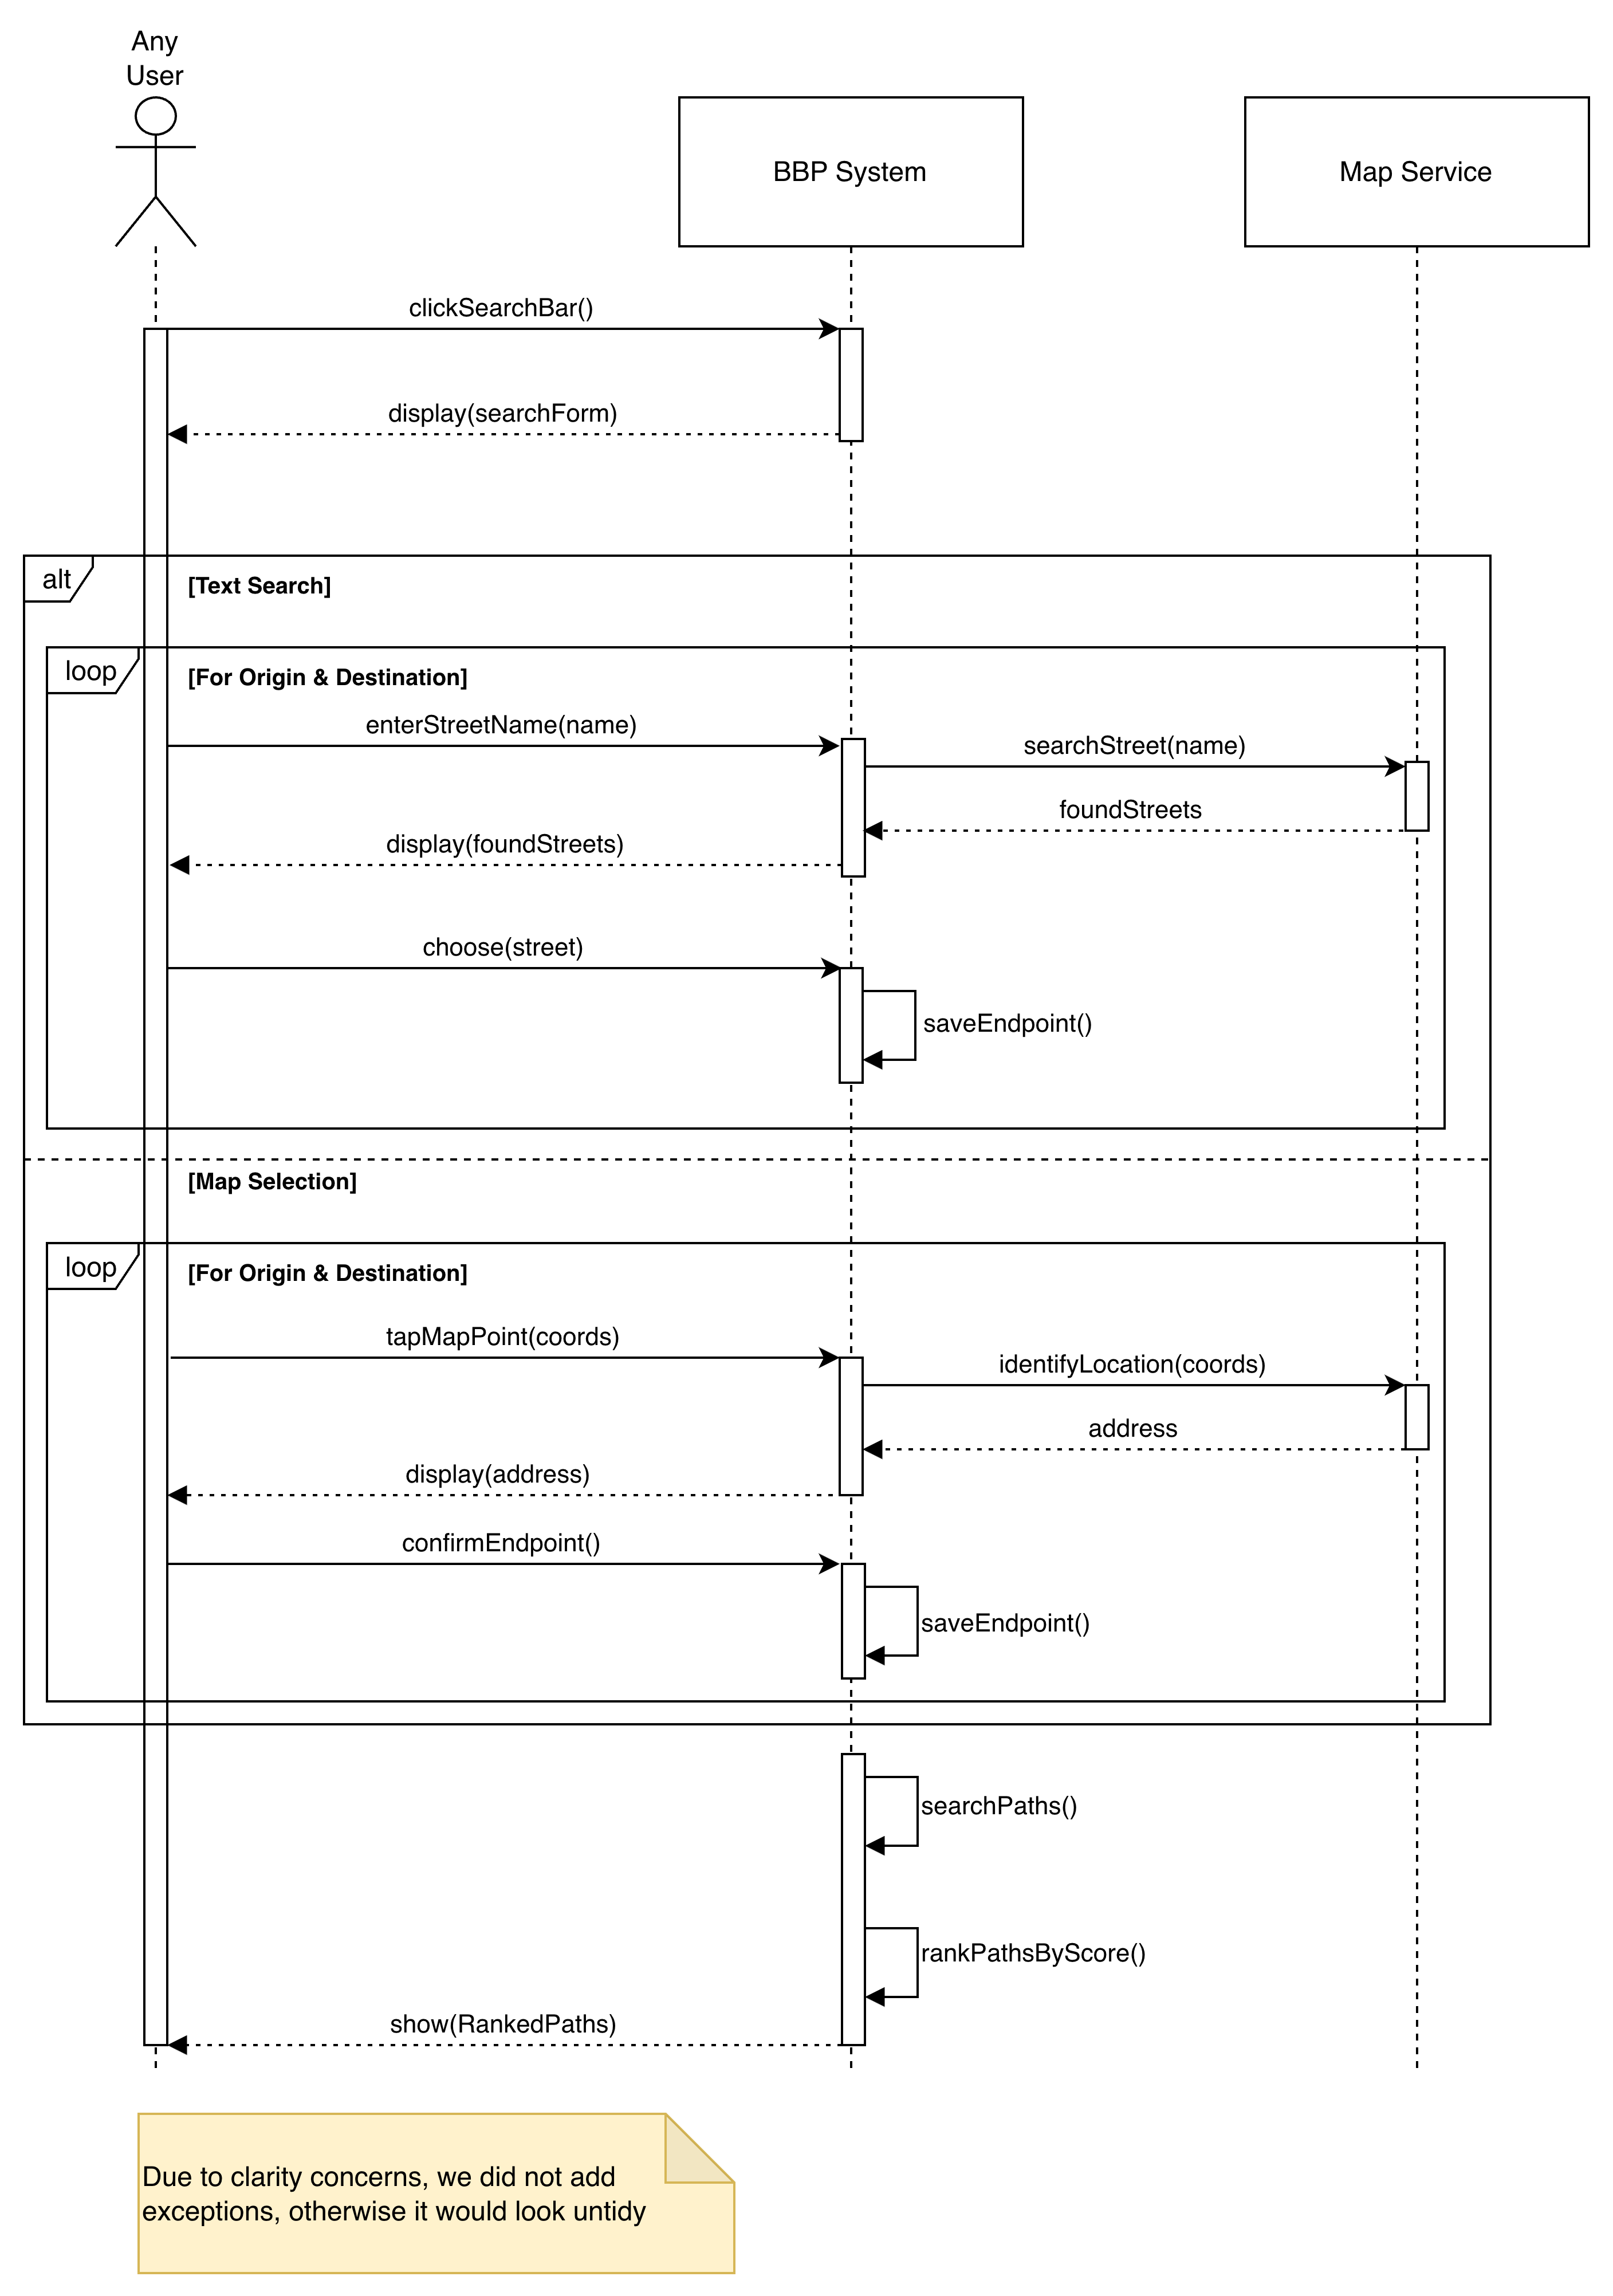
\includegraphics[width=\textwidth]{diagrams/sequence diagrams/uc9.png}
    \caption{Sequence Diagram for UC9: Search Path}
    \label{fig:uc9_sequence}
\end{figure}


\begin{table}[H]
\centering
\begin{tabularx}{\textwidth}{|l|X|}
\hline
\multicolumn{2}{|c|}{\textbf{[UC10] - Visualize Path}} \\ \hline
\textbf{Participating Actors} & \texttt{User}, \texttt{Map Service}, \texttt{Weather Service} \\ \hline
\textbf{Entry condition}      & The User has searched paths between two points and has chosen one listed option. \\ \hline
\textbf{Flow of events}       & 
\begin{enumerate}
    \item The \texttt{User} clicks on one path in the search results list.
    \item \texttt{BBP} queries the \texttt{Map Service} to fetch map data and \texttt{GPS coordinates} for the chosen path.
    \item \texttt{BBP} queries the \texttt{Weather Service} for current environmental conditions along the selected path.
    \item \texttt{BBP} displays a detailed view showing the path \texttt{trajectory} on the map, aggregated statistics (\texttt{average time}, \texttt{total distance}, and \texttt{status}), confirmed potholes, and current weather conditions along the path.
\end{enumerate} \\ \hline
\textbf{Exit conditions}      & The user is shown the path on the map interface along with its aggregated statistics and current weather conditions. \\ \hline
\textbf{Exceptions}           & 
\textbf{Weather Service Unavailable:} \texttt{BBP} displays an error notification regarding the weather data but continues to load the map and statistics. \newline
\textbf{Map Service Unavailable:} \texttt{BBP} shows an error and suggests trying again later  \\ \hline
\end{tabularx}
\caption{Use Case 10: Visualize Path}
\label{tab:uc10}
\end{table}

\begin{figure}[H]
    \centering
    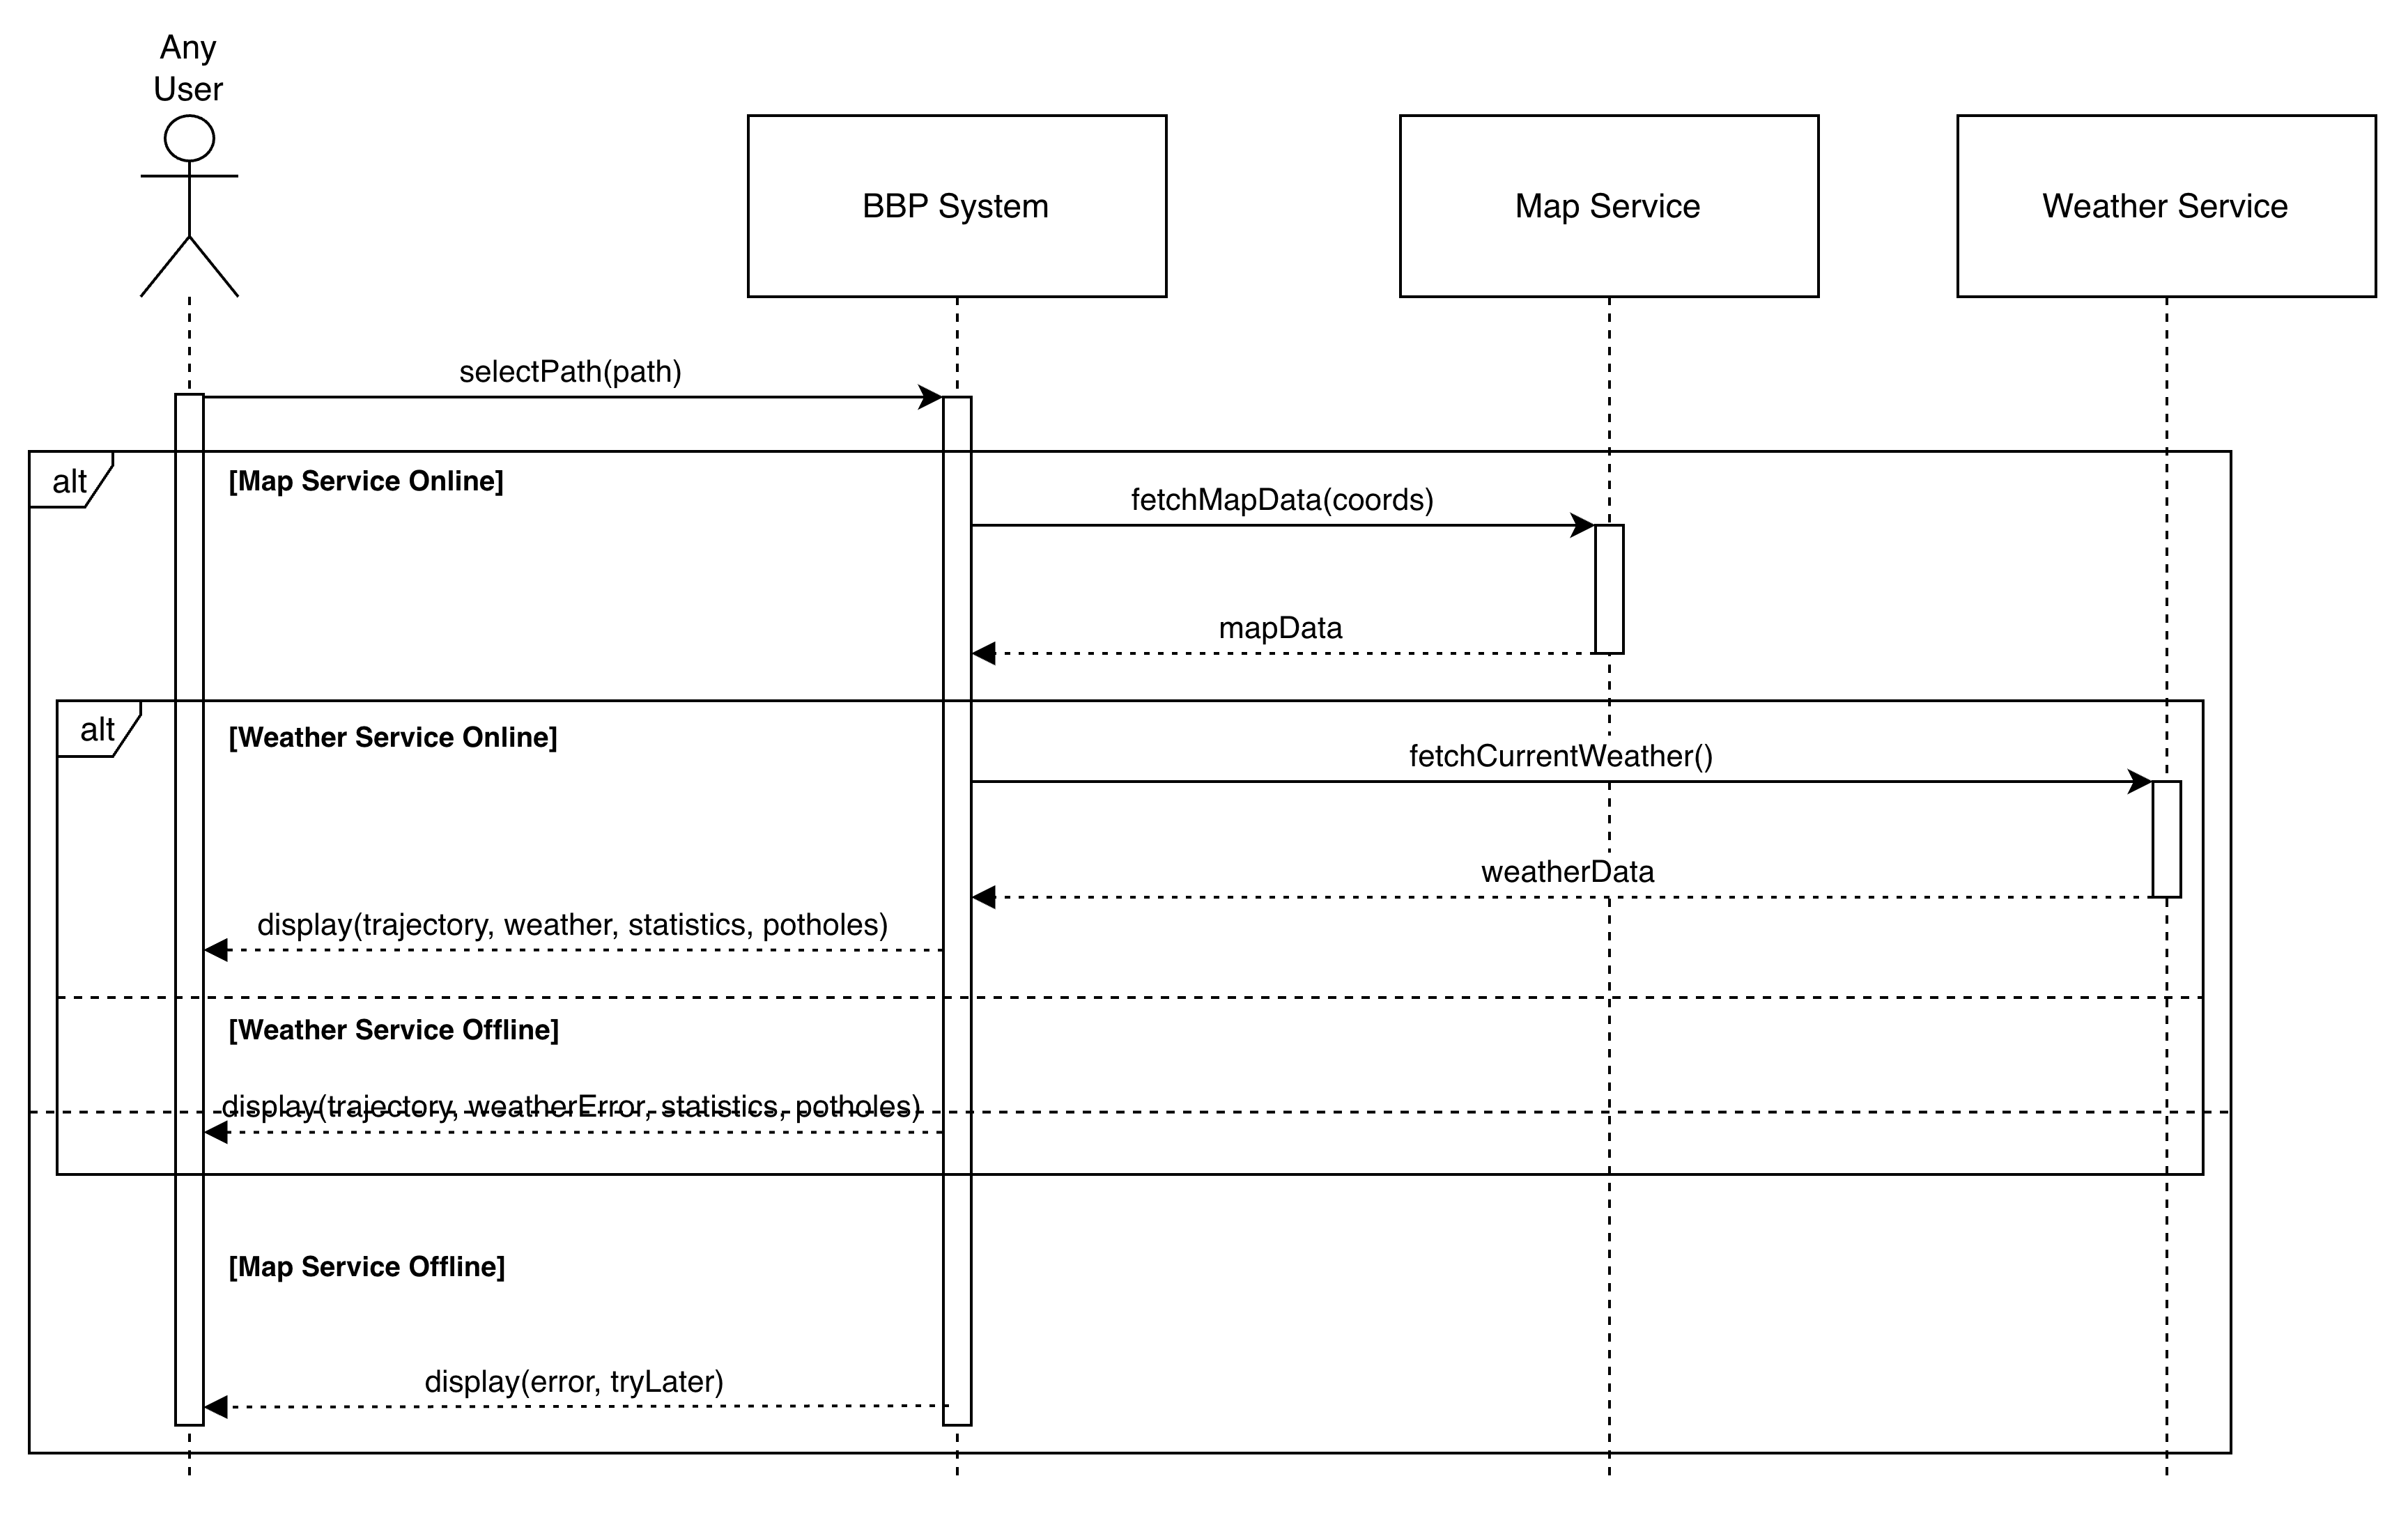
\includegraphics[width=\textwidth]{diagrams/sequence diagrams/uc10.png}
    \caption{Sequence Diagram for UC10: Visualize Path}
    \label{fig:uc10_sequence}
\end{figure}

\subsection{Requirements Mapping}

% --- GOAL 0 ---
\begin{table}[htbp]
\centering
\begin{tabular}{|p{2.5cm}|p{1cm}|p{10.5cm}|}
\hline
\multicolumn{3}{|c|}{\textbf{G0 - A user wants to signup first and then login to the application.}} \\
\hline
\textbf{Use Cases} & \multicolumn{2}{c|}{\textbf{Requirements and Domain Assumptions}} \\
\hline
UC1 & \textbf{R1} & The system must allow an unregistered User to sign up. \\
\hline
UC2 & \textbf{R2} & The system must allow registered Users to login. \\
\hline
\end{tabular}
\end{table}

% --- GOAL 1 ---
\begin{longtable}{|p{2.5cm}|p{1cm}|p{10.5cm}|}
\hline
\multicolumn{3}{|p{14.5cm}|}{\centering \textbf{G1 - A registered user aims to automatically record their cycling trips using theirs
mobile device’s sensors.}} \\
\hline
\textbf{Use Cases} & \multicolumn{2}{c|}{\textbf{Requirements and Domain Assumptions}} \\
\hline
& \textbf{D.1.1} & \textbf{Sensor Reliability}: It is assumed that GPS, accelerometer and gyroscope
sensors provided by the mobile hardware are sufficiently precise to distinguish biking
vibrations from road anomalies effectively. \\
\hline
& \textbf{D.1.2} & \textbf{Biking Speed Distinctiveness}: It is assumed that the speed and the
acceleration of a user cycling are mathematically distinguishable from those of walk-
ing, running or driving a car, enabling the Automated Mode to function correctly
without explicit user triggers. \\
\hline
UC1 & \textbf{R1} & The system must allow an unregistered User to sign up. \\
\hline
UC2 & \textbf{R2} & The system must allow registered Users to login. \\
\hline
UC3 & \textbf{R4} & The system must allow a Registered User to automatically record a trip using device sensors. \\
\hline
UC3 & \textbf{R5} & The system must allow the Registered User to start and stop the process by pressing buttons. \\
\hline
UC3 & \textbf{R6} & The system must automatically start (or resume) the sensors tracking when cycling activity is detected and pause it when the user stops cycling.\\
\hline
UC3 &\textbf{R7} & The system must analyze sensors' data to detect potential anomalies (e.g., potholes).\\
\hline
UC3     &\textbf{R8} & The system must produce trip statistics (distance, average speed, duration and weather conditions at the time of recording) and append them to trip information.\\
\hline
UC3     &\textbf{R9} & The system must buffer trip data locally and synchronize it with the server once trip recording has ended in order to overcome network connectivity unavailability.\\
\hline
UC3     &\textbf{R10} & In case of anomalies detection, the system must allow a Registered User to confirm or reject each detected anomaly within 72 hours from the trip recording.\\
\hline
UC3     &\textbf{R11} & The system shall allow Registered Users to publish validated trips in an anonymized form to protect user privacy.\\
\hline
\end{longtable}

\vspace{0.6cm}

% --- GOAL 2 ---
\begin{longtable}{|p{2.5cm}|p{1cm}|p{10.5cm}|}
\hline
\multicolumn{3}{|p{14.5cm}|}{\centering \textbf{G2 - A registered user aims to manually record a bike trip by inserting one street at a time without physical cycling.}} \\
\hline
\textbf{Use Cases} & \multicolumn{2}{c|}{\textbf{Requirements and Domain Assumptions}} \\
\hline
UC1 & \textbf{R1} & The system must allow an unregistered User to sign up. \\
\hline
UC2 & \textbf{R2} & The system must allow registered Users to login. \\
\hline
UC4 & \textbf{R3} & The system must allow a Registered User to manually insert a bike trip by listing the name and the status of each street comprising the trip. \\
\hline
\end{longtable}

\vspace{0.5cm}

% --- GOAL 3 ---
\begin{longtable}{|p{2.5cm}|p{1cm}|p{10.5cm}|}
\hline
\multicolumn{3}{|p{14.5cm}|}{\centering \textbf{G3 - A registered user wants to access their recorded bike trips history}} \\
\hline
\textbf{Use Cases} & \multicolumn{2}{c|}{\textbf{Requirements and Domain Assumptions}} \\
\hline
UC1 & \textbf{R1} & The system must allow an unregistered User to sign up. \\
\hline
UC2 & \textbf{R2} & The system must allow registered Users to login. \\
\hline
UC3, UC4 & \textbf{R12} & The system must allow Registered Users to store all their recorded trips (manually or automatically). \\
\hline
UC7 & \textbf{R13} & The system must allow a Registered User to view his private trip history. \\
\hline
\end{longtable}

\vspace{0.5cm}

% --- GOAL 4 ---
\begin{longtable}{|p{2.5cm}|p{1cm}|p{10.5cm}|}
\hline
\multicolumn{3}{|p{14.5cm}|}{\centering \textbf{G4 - A registered user aims to view trip on map and consult its statistics, including average speed, trip time and meteorological conditions (at recording time)}} \\
\hline
\textbf{Use Cases} & \multicolumn{2}{c|}{\textbf{Requirements and Domain Assumptions}} \\
\hline
UC1 & \textbf{R1} & The system must allow an unregistered User to sign up. \\
\hline
UC2 & \textbf{R2} & The system must allow registered Users to login. \\
\hline
UC3 & \textbf{R8} & The system must produce trip statistics (distance, average speed, duration and weather conditions at the time of recording) and append them to trip information. \\
\hline
UC7 & \textbf{R13} & The system must allow a Registered User to view his private trip history. \\
\hline
UC7 & \textbf{R14} & The system must allow a Registered User to review the statistics related to a bike trip, such as average speed, total distance and weather conditions when available. \\
\hline
\end{longtable}

\newpage

% --- GOAL 5 ---
\begin{longtable}{|p{2.5cm}|p{1cm}|p{10.5cm}|}
\hline
\multicolumn{3}{|p{14.5cm}|}{\centering \textbf{G5 - A registered user wants to share information about a bike trip they have recorded, including their status and the presence of obstacles, making this information available to the community (all users).}} \\
\hline
\textbf{Use Cases} & \multicolumn{2}{c|}{\textbf{Requirements and Domain Assumptions}} \\
\hline
UC1 & \textbf{R1} & The system must allow an unregistered User to sign up. \\
\hline
UC2 & \textbf{R2} & The system must allow registered Users to login. \\
\hline
UC5 & \textbf{R10} & In case of anomalies detection, the system must allow a Registered User to confirm or reject each detected anomaly within 72 hours from the trip recording. \\
\hline
UC6 & \textbf{R11} & The system shall allow Registered Users to publish validated trips in an anonymized form to protect user privacy. \\
\hline
UC7 & \textbf{R13} & The system must allow a Registered User to view his private trip history. \\
\hline
UC7 & \textbf{R14} & The system must allow a Registered User to review the statistics related to a bike trip, such as average speed, total distance and weather conditions when available. \\
\hline
\end{longtable}

\vspace{0.5cm}

% --- GOAL 6 ---
\begin{longtable}{|p{2.5cm}|p{1cm}|p{10.5cm}|}
\hline
\multicolumn{3}{|p{14.5cm}|}{\centering \textbf{G6 - A User wants to search for bike paths given an origin and a destination point and visualize results on a map.}} \\
\hline
\textbf{Use Cases} & \multicolumn{2}{c|}{\textbf{Requirements and Domain Assumptions}} \\
\hline
UC9 & \textbf{R15} & The system must allow any User to search for bike paths between a given origin and a given destination. \\
\hline
UC9 & \textbf{R16} & The system must list and rank available paths based on their Path Score. \\
\hline
UC9 & \textbf{R17} & The system must visualize available paths on a map \\
\hline
UC6 & \textbf{R18} & The system must compute a Path Score based on Path status and estimated trip time (effectiveness). \\
\hline
\end{longtable}

\vspace{0.5cm}

% --- GOAL 7 ---
\begin{longtable}{|p{2.5cm}|p{1cm}|p{10.5cm}|}
\hline
\multicolumn{3}{|p{14.5cm}|}{\centering \textbf{G7 - A User wants to retrieve up-to-date information about bike paths, their status, and current weather conditions.}} \\
\hline
\textbf{Use Cases} & \multicolumn{2}{c|}{\textbf{Requirements and Domain Assumptions}} \\
& \textbf{D.1.3} & \textbf{User Trustworthiness:} Given the community-based nature of the data,
it is assumed that Registered Users will generally provide truthful validations regarding obstacles and path status. \\
\hline
& \textbf{D.1.4} & \textbf{Obstacle Detection:} If different Automatic Trips corresponding to the same Path detect the same obstacle, we assume that the obstacle has the same
coordinates in both trips. \\
\hline
UC10 & \textbf{R19} & The system must allow any User to view public Path information such as aggregated statistics such as status, total distance, average trip time, and merged anomalies. \\
\hline
UC10 & \textbf{R20} & The system shall query an external weather service to retrieve current weather conditions during the path visualization. \\
\hline
UC6 & \textbf{R21} & The system must merge published information from multiple Users referring to the same path, considering their freshness and the number of confirming contributions. \\
\hline
UC6 & \textbf{R22} & The system must remove obstacles from a path when newer published trips covering the same trajectory do not report those obstacles, maintaining data consistency with current road conditions. \\
\hline
\hline
\end{longtable}

% --- GOAL 8 ---
\begin{longtable}{|p{2.5cm}|p{1cm}|p{10.5cm}|}
\hline
\multicolumn{3}{|p{14.5cm}|}{\centering \textbf{G8 - A registered user wants to delete one of their previously recorded trips.}} \\
\hline
\textbf{Use Cases} & \multicolumn{2}{c|}{\textbf{Requirements and Domain Assumptions}} \\
\hline
UC1 & \textbf{R1} & The system must allow an unregistered User to sign up. \\
\hline
UC2 & \textbf{R2} & The system must allow registered Users to login. \\
\hline
UC3, UC4 & \textbf{R12} & The system must allow Registered Users to store all their recorded trips (manually or automatically). \\
\hline
UC7 & \textbf{R13} & The system must allow a Registered User to view his private trip history. \\
\hline
UC8 & \textbf{R23} & The system must allow a Registered User to delete one of their recorded trips.\\
\hline
\end{longtable}


\section{Performance Requirements}
\label{sec:performance}

To ensure an optimal user experience, the system should complete actions within 2 seconds. However for this application, that does not involve critical services, strict requirements are not needed. For this reason completion time for complex tasks can be extended up to 5 seconds. Those complex tasks could be:

\begin{itemize}
    \item searching and displaying available paths
    \item calculating and displaying statistical information
\end{itemize}

\section{Design Constraints}
\label{sec:constraints}

\subsection{Standards Compliance}

Since the system collects and stores sensitive user data, the design must strictly adhere to the General Data Protection Regulation (GDPR). This includes implementing mechanisms for:
\begin{itemize}
    \item Explicit user consent for tracking.
    \item The deletion of all user data upon request.
    \item Anonymization of data when aggregated for public statistics.
\end{itemize}

\subsection{Hardware Limitations}

\begin{itemize}
    \item \textbf{Mandatory Sensor Availability}: The automated tracking module is constrained by the physical hardware of the user's device. The application cannot function in automated mode on devices lacking working sensors such as GPS, accelerometer, gyroscope.

    \item \textbf{Local Storage Capacity}: The local buffering feature for offline recording is constrained by the available internal storage of the mobile device. The application design must include a safe upper limit for the buffer size to avoid filling the user's device storage.

    \item \textbf{Battery Drain Constraints}: The software must use optimizations techniques or/and APIs to minimize battery usage.
\end{itemize}

\subsection{Implementation Constraints}

\begin{itemize}
    \item \textbf{Third-party APIs Limits}: The design is constrained by the Rate Limits imposed by external service providers. The software must implement some strategies to avoid exceeding Rate Limits and incurring service denials or extra costs.
\end{itemize}

\section{Software System Attributes}
\label{sec:attributes}

\subsection{Reliability}

To ensure better reliability performance, regular maintenance and bug fixes should be performed. Planned maintenance should also be notified to users to avoid any unexpected inconvenience.

\subsection{Availability}

To ensure a positive user experience, the system uptime should be 99\% or more. This application does not involve critical tasks (e.g., financial transactions) so the minimum standard it's not required to be 99.5\% or more.

The core function of trip recording in automated mode should be available 100\% of the time, regardless of network status, provided the device has sufficient battery and storage.

\subsection{Security}

The system shall enforce strict access control policies. A user's specific history and sensor logs must be accessible only to that specific user, unless explicitly published.

User passwords shall never be stored in plain text. The system must use industry-standard hashing algorithms with unique salts for credential storage.

\subsection{Maintainability}

The architecture should follow a modular approach to facilitate debugging and programming.

The source code should also be documented following standard conventions (e.g., Javadoc for Java, PyDoc for Python) to facilitate future maintenance and onboarding of new developers.

\subsection{Portability}

BBP is a mobile application so it has to be compatible with both major OSs (Android and iOS).
